\chapter{Referencia técnica}
\label{chap:ref-tecnica}

\lettrine{E}{n} este apéndice se reflejan las distintas referencias técnicas del \acrshort{tfg}:

\begin{itemize}
\item Casos de uso
\item Diagrama entidad-relación
\item Estructura del código
\end{itemize}

\section{Casos de uso}
\label{chap:casos-uso}

Se definen tres tipos de usuarios de la aplicación en función de los funcionalidades que puedan realizar en la misma en función del perfil que tengan asignado. Los perfiles defindos para la aplicación son los siguientes:

\begin{itemize}
\item READ: perfil de sólo lectura. Sólamente permite visualizar la información almacenada en la aplicación, pero no puede realizar ninguna modificación, salvo la relativa a su información de contacto y su contraseña.
\item MODIF: perfil de lectura y modificación. Además de las funcionalidades descritas para el perfil READ, permite realizar modificaciones sobre las distintas entidades del sistema (altas/bajas/modificaciones).
\item ADMIN: perfil de administrador. Además de las funcionalidades descritas para el perfil WRITE, permite la gestión de usuarios (altas/bajas/modificaciones).
\end{itemize}


\subsection{Actores}
\label{sub:actores}


\begin{figure}[hp!]
  \centering
  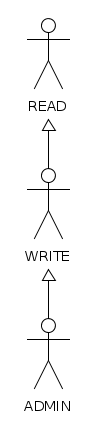
\includegraphics[width=0.05\textwidth]{imaxes/actores.png}
  \caption{Actores del sistema}
  \label{fig:actores}
\end{figure}

El actor ADMIN representa a los usuarios de la aplicación que tienen
acceso completo a todas las funciones, incluyendo la gestión de usuarios.

Los actores  READ y  WRITE representa a cualquier usuario con un perfil READ o MODIF, respectivamente, que haya sido dado de alta previamente por un actor ADMIN, que representa a cualquier usuario con perfil ADMIN, y disponga de un nombre de usuario y una contraseña.




\subsection{Casos de uso}
\label{sub:casos-uso}


Todos los usuarios comparten los casos de uso de acceso y los relativos a la consulta de las entidades del sistema. El actor WRITE amplía esos casos de uso con funcionalidades de creación, modificación y borrado de entidades y por último el actor ADMIN amplía esos casos de uso con el caso de uso de administración de usuarios. Las siguientes figuras (\ref{fig:cu-acceso}, \ref{fig:cu-read-write}, \ref{fig:cu-admin} de las páginas \ref{fig:cu-acceso},\ref{fig:cu-read-write},\ref{fig:cu-admin}) muestran una visión de alto nivel de los distintos casos de uso definidos en el sistema. Dichos casos de uso se analizan con más detalle en los siguientes apartados.


\begin{figure}[hp!]
  \centering
  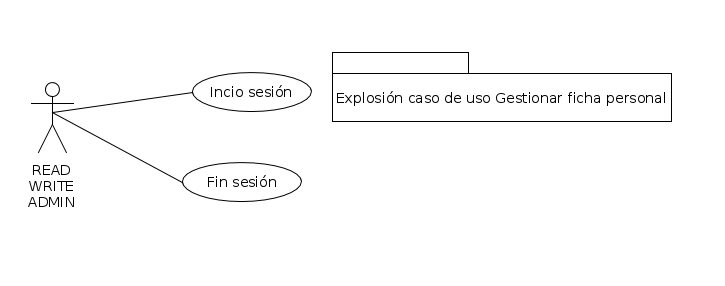
\includegraphics[width=0.50\textwidth]{imaxes/cu_acceso.png}
  \caption{Caso de uso del acceso al sistema - Actores READ, WRITE y ADMIN}
  \label{fig:cu-acceso}
\end{figure}



\begin{figure}[hp!]
  \centering
  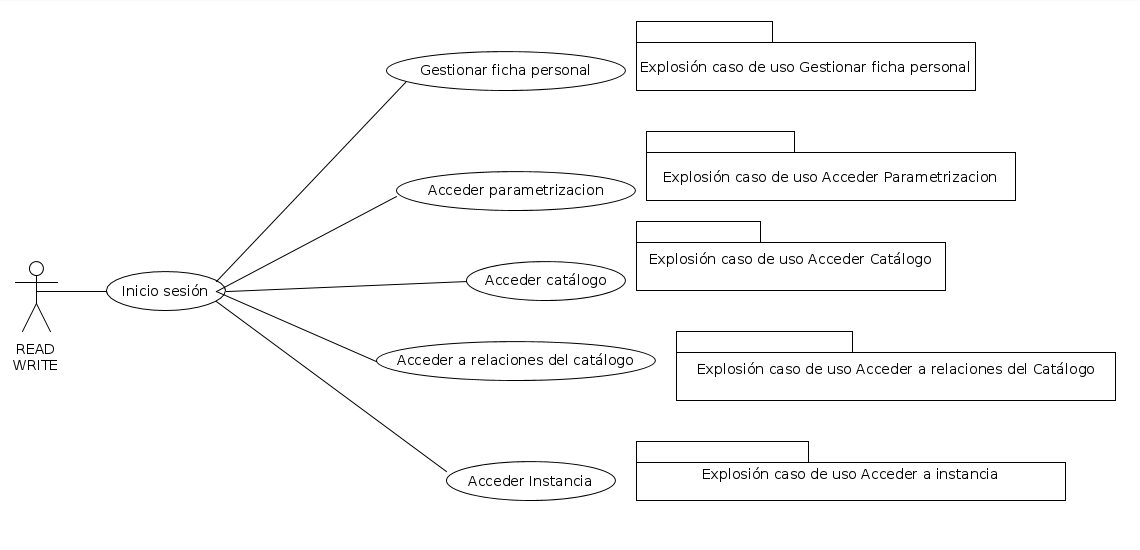
\includegraphics[width=0.50\textwidth]{imaxes/cu-read-write.png}
  \caption{Casos de uso de los actores READ, WRITE}
  \label{fig:cu-read-write}
\end{figure}


\begin{figure}[hp!]
  \centering
  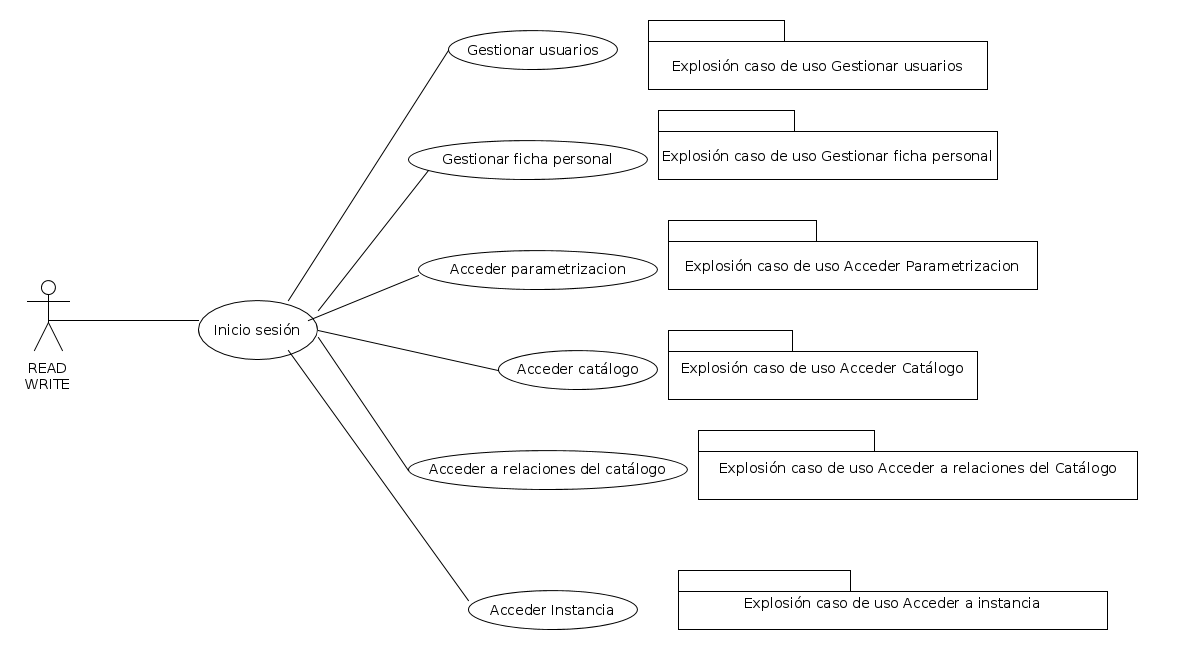
\includegraphics[width=0.50\textwidth]{imaxes/cu-admin.png}
  \caption{Casos de uso del actor ADMIN}
  \label{fig:cu-admin}
\end{figure}




\subsubsection{Caso de uso de acceso al sistema} 
\label{sub:cu-acceso}

Para poder accede al sistema es necesario que el usuario esté dado de alta y disponga de un usuario y contraseña válidos. Desde el punto de vista del acceso existen dos casos de uso: inicio de sesión (\ref{tab:cu-inicio-sesion}, página \pageref{tab:cu-inicio-sesion}) y término de sesión(\ref{tab:cu-fin-sesion}, página \pageref{tab:cu-fin-sesion}).



\begin{table} [H]
    \centering
    \rowcolors{2}{white}{white}
    \setlength{\leftmargini}{0.4cm}
	\resizebox{14cm}{!} { % evita que la tabla sobresalga de la p\'agina, ajustando tama\'no de letra y grosor de l\'ineas
    \begin{tabular}{| m{3cm} | m{11cm} |}   
    \hline
	  \textbf{CU-01} & \textbf{Inicio de sesión} \\\hline
	  \textbf{Descripción} & Permite el acceso del usuario a la aplicación. \\\hline
	  \textbf{Actores} & READ, WRITE y ADMIN. \\\hline
	  \textbf{Precondiciones} & El usuario no tiene sesión iniciada. \\\hline
	  \textbf{Postcondiciones} & Se crea una nueva sesión en el sistema para el usuario. \\\hline
	  \textbf{Flujo básico} & 
		\begin{enumerate}
	  	\item El sistema muestra un formulario con campos de nombre de usuario y contraseña y un botón de envío de los datos del formulario.
		\item El usuario cubre el formulario con los datos correspondientes y envía la información del mismo a través del botón de envío.
	  	\item El sistema valida los datos de conexión del usuario, le crea una nueva sesión y lo redirige a la página principal.	
	  	\begin{enumerate}
		   \item \textit{\textbf{Flujo alternativo:} Si el usuario no existe, o la contraseña no es correcta, el sistema informa del
error y se reinicia el caso de uso.}
		\end{enumerate}   	
	   	\item Finaliza el caso de uso.
	  \end{enumerate} 	  	  
	  \\\hline
    \end{tabular}
    } % end /resizebox
    \caption{CU-01 Inicio de sesión}
    \label{tab:cu-inicio-sesion}
\end{table}




\begin{table} [H]
    \centering
    \rowcolors{2}{white}{white}
    \setlength{\leftmargini}{0.4cm}
	\resizebox{14cm}{!} { % evita que la tabla sobresalga de la p\'agina, ajustando tama\'no de letra y grosor de l\'ineas
    \begin{tabular}{| m{3cm} | m{11cm} |}   
    \hline
	  \textbf{CU-02} & \textbf{Fin de sesión} \\\hline
	  \textbf{Descripción} & Permite al usuario terminar la sesión previamente iniciada y desconectarse del sistema. \\\hline
	  \textbf{Actores} & READ, WRITE y ADMIN. \\\hline
	  \textbf{Precondiciones} & El usuario se encuentra conectado actualmente. \\\hline
	  \textbf{Postcondiciones} & Se finaliza la sesión de usuario y se eliminan los recursos asociados. \\\hline
	  \textbf{Flujo básico} & 
		\begin{enumerate}
	  	\item El usuario da orden de finalizar la sesión mediante un botón de fin de sesión.
		\item El sistema finaliza la sesión del usuario y descarta todos los datos asociados.
	  	\item El sistema redirige al usuario hacia la pantalla inicial de acceso a la aplicación.		  
	   	\item Finaliza el caso de uso.
	  \end{enumerate} 	  	  
	  \\\hline
    \end{tabular}
    } % end /resizebox
    \caption{CU-02 Fin de sesión}
    \label{tab:cu-fin-sesion}
\end{table}




\subsubsection{Casos de uso genéricos (búsqueda, creación, edición, borrado, etc.} 
\label{sub:cu-genericos}

En este apartado se muestran los casos de uso genéricos para la búsqueda, selección, creación, edición y borrado de los distintos elementos del sistema.

%%%%%%%%%%%%%%%%%%%%%%%%%%%%%%%%%%%%%%%%%%
%% CASOS DE USO GENÉRICOS PARA CREACIÓN %%
%%%%%%%%%%%%%%%%%%%%%%%%%%%%%%%%%%%%%%%%%%

\begin{table} [H]
    \centering
    \rowcolors{2}{white}{white}
    \setlength{\leftmargini}{0.4cm}
	\resizebox{14cm}{!} { % evita que la tabla sobresalga de la p\'agina, ajustando tama\'no de letra y grosor de l\'ineas
    \begin{tabular}{| m{3cm} | m{11cm} |}   
    \hline
	  \textbf{CU-03} & \textbf{Crear nuevo elemento} \\\hline
	  \textbf{Descripción} & Crear nuevo elemento. \\\hline
	  \textbf{Actores} & WRITE y ADMIN. \\\hline
	  \textbf{Precondiciones} & El usuario del actor WRITE o ADMIN ha pulsado el botón de crear nueva entidad. \\\hline
	  \textbf{Postcondiciones} & Se añade un nuevo registro en el listado de la entidad. \\\hline
	  \textbf{Flujo básico} & 
		\begin{enumerate}
	  	\item El sistema muestra un cuadro de dialogo con los campos que describen el elemento.
\item El usuario rellena los campos deseados. Pulsa el botón de guardar.
\item El sistema comprueba que los campos obligatorios han sido completados y que los datos tienen el formato correcto. Se guardan los datos de fecha de creación y nombre de usuario, se añade al listado de la entidad, se informa al usuario que el ítem ha sido añadido y se cierra el cuadro de diálogo.
			\begin{enumerate}	
			   \item \textit{\textbf{Flujo alternativo:} Si no se cubre algún campo obligatorio o se produce algún error de validación el sistema informa del error.}			   
			\end{enumerate}
\item Finaliza el caso de uso.
	  \end{enumerate} 	  	  
	  \\\hline
    \end{tabular}
    } % end /resizebox
    \caption{CU-03 Crear nueva entidad de parametrización}
    \label{tab:cu-nuevo-elemento}
\end{table}

%%%%%%%%%%%%%%%%%%%%%%%%%%%%%%%%%%%%%%%%%
%% CASOS DE USO GENÉRICOS PARA EDICIÓN %%
%%%%%%%%%%%%%%%%%%%%%%%%%%%%%%%%%%%%%%%%%

\begin{table} [H]
    \centering
    \rowcolors{2}{white}{white}
    \setlength{\leftmargini}{0.4cm}
	\resizebox{14cm}{!} { % evita que la tabla sobresalga de la p\'agina, ajustando tama\'no de letra y grosor de l\'ineas
    \begin{tabular}{| m{3cm} | m{11cm} |}   
    \hline
	  \textbf{CU-04} & \textbf{Editar elemento seleccionado} \\\hline
	  \textbf{Descripción} & Editar elemento seleccionado. \\\hline
	  \textbf{Actores} & WRITE y ADMIN. \\\hline
	  \textbf{Precondiciones} & El usuario del actor WRITE o ADMIN ha pulsado el botón editar para un elemento de la entidad. \\\hline
	  \textbf{Postcondiciones} & Se modifica el elemento del listado de la entidad. \\\hline
	  \textbf{Flujo básico} & 
		\begin{enumerate}
	  	\item El sistema muestra los campos editables del registro seleccionado y dos botones: guardar y cancelar.
\item El usuario modifica los campos deseados sobre el registro. 
			\begin{enumerate}	
			   \item El usuario pulsa el botón de guardar. El sistema comprueba que los campos obligatorios han sido completados y que los datos tienen el formato correcto. Se guardan los datos de fecha de creación y nombre de usuario. Se termina la edición del registro. Se informa al usuario que el ítem ha sido modificado. Se actualiza el listado de la entidad con las modificaciones realizadas.
			   \begin{enumerate}	
			   \item  \textit{\textbf{Flujo alternativo:} Si no se cubre algún campo obligatorio o se produce algún error de validación el sistema informa del error.}
			   \end{enumerate}
			   \item El usuario pulsa el botón cancelar. Se termina la edición del registro y se descartan los posibles cambios.
			\end{enumerate}
	  \item Finaliza el caso de uso.
	  \end{enumerate} 	  	  
	  \\\hline
    \end{tabular}
    } % end /resizebox
    \caption{CU-04 Editar elemento seleccionado}
    \label{tab:cu-editar-elemento}
\end{table}


\begin{table} [H]
    \centering
    \rowcolors{2}{white}{white}
    \setlength{\leftmargini}{0.4cm}
	\resizebox{14cm}{!} { % evita que la tabla sobresalga de la p\'agina, ajustando tama\'no de letra y grosor de l\'ineas
    \begin{tabular}{| m{3cm} | m{11cm} |}   
    \hline
	  \textbf{CU-05} & \textbf{Editar registro de histórico del elemento seleccionado} \\\hline
	  \textbf{Descripción} & Editar registro de histórico del elemento seleccionado. \\\hline
	  \textbf{Actores} & WRITE y ADMIN. \\\hline
	  \textbf{Precondiciones} & El usuario del actor WRITE o ADMIN ha pulsado el botón editar para el registro de histórico para el elemento seleccionado. \\\hline
	  \textbf{Postcondiciones} & Se modifica el registro de histórico elemento del listado de la entidad  y, si es necesario, se modifican las fechas de los regisros registros anterior y posterior para que sean consecutivos. \\\hline
	  \textbf{Flujo básico} & 
		\begin{enumerate}
	  	\item El sistema muestra los campos editables del registro seleccionado y dos botones: guardar y cancelar.
        \item El usuario modifica los campos deseados sobre el registro. Si el estado del registro cambia al estado cancelado se dispara el caso de uso \ref{tab:cu-cancelar-historico} (página \pageref{tab:cu-cancelar-historico}).
			\begin{enumerate}	
			   \item El usuario pulsa el botón de guardar. El sistema comprueba que los campos obligatorios han sido completados y que los datos tienen el formato correcto. Realiza las modificaciones pertinentes en los registros de histórico anterior y posterior del elemento seleccionado, de forma que todos los registros de histórico sean correlativos. Se guardan los datos de fecha de creación y nombre de usuario tanto para el nuevo registro de histórico como para los registros adyacentes modificados. Se termina la edición del registro. Se informa al usuario que el registro ha sido modificado y se actualiza el listado de la entidad con las modificaciones realizadas.
			   \begin{enumerate}	
			   \item  \textit{\textbf{Flujo alternativo:} Si no se cubre algún campo obligatorio o se produce algún error de validación el sistema informa del error.}
			   \end{enumerate}
			   \item El usuario pulsa el botón cancelar. Se termina la edición del registro y se descartan los posibles cambios.
			\end{enumerate}
	  \item Finaliza el caso de uso.
	  \end{enumerate} 	  	  
	  \\\hline
    \end{tabular}
    } % end /resizebox
    \caption{CU-05 Editar histórico de elemento seleccionado}
    \label{tab:cu-editar-historico}
\end{table}

\begin{table} [H]
    \centering
    \rowcolors{2}{white}{white}
    \setlength{\leftmargini}{0.4cm}
	\resizebox{14cm}{!} { % evita que la tabla sobresalga de la p\'agina, ajustando tama\'no de letra y grosor de l\'ineas
    \begin{tabular}{| m{3cm} | m{11cm} |}   
    \hline
	  \textbf{CU-06} & \textbf{Cancelar el registro de histórico del elemento seleccionado} \\\hline
	  \textbf{Descripción} & Cancelar el registro de histórico del elemento seleccionado. \\\hline
	  \textbf{Actores} & WRITE y ADMIN. \\\hline
	  \textbf{Precondiciones} & El usuario del actor WRITE o ADMIN ha seleccionado el estado cancelado para el registro de histórico que está modificando. \\\hline
	  \textbf{Postcondiciones} & Se propaga el estado de cancelado para todos los registros de histórico posteriores al registro seleccionado. \\\hline
	  \textbf{Flujo básico} & 
		\begin{enumerate}
	  	\item Se muestra un cuadro de diálogo solicitando propagar el estado cancelado para los registros posteriores al registro de histórico seleccionado.
        \item 
			\begin{enumerate}	
			   \item El usuario pulsa el botón de aceptar. El sistema propaga el nuevo estado al resto de registros de históricos posteriores al registro de histórico seleccionado. Se cierra el cuadro de diálogo.
			   \item El usuario pulsa el botón cancelar. Se cierra el cuadro de diálogo y se descarta el cambio de estado.
			\end{enumerate}
	  \item Finaliza el caso de uso.
	  \end{enumerate} 	  	  
	  \\\hline
    \end{tabular}
    } % end /resizebox
    \caption{CU-06 Cancelar el registro de histórico del elemento seleccionado}
    \label{tab:cu-cancelar-historico}
\end{table}




\begin{table} [H]
    \centering
    \rowcolors{2}{white}{white}    
    \setlength{\leftmargini}{0.4cm}
	\resizebox{14cm}{!} { % evita que la tabla sobresalga de la p\'agina, ajustando tama\'no de letra y grosor de l\'ineas
    \begin{tabular}{| m{3cm} | m{11cm} |}   
    \hline
	  \textbf{CU-07} & \textbf{Añadir registro de histórico del elemento seleccionado} \\\hline
	  \textbf{Descripción} & Añadir registro de histórico del elemento seleccionado. \\\hline
	  \textbf{Actores} & WRITE y ADMIN. \\\hline
	  \textbf{Precondiciones} & El usuario del actor WRITE o ADMIN ha pulsado el botón añadir registro de histórico para el elemento seleccionado. \\\hline
	  \textbf{Postcondiciones} & Se añade un nuevo registro de histórico  comprendido entre el elemento seleccionado del listado de la entidad y el siguiente elemento de la lista, o a continuación del elemento seleccionado si no hay más elementos en la lista, modificando fechas de dichos regisros para que sean consecutivos. \\\hline
	  \textbf{Flujo básico} & 
		\begin{enumerate}
	  	\item El sistema muestra un formulario con una copia del registro de histórico del elemento seleccionado con los campos susceptibles de modificar habilitados. El usuario modificará las fechas de inicio y/o fin del registro, así como el resto de campos que considere oportuno. 
			\begin{enumerate}	
			   \item El usuario pulsa el botón de guardar. El sistema comprueba que los campos obligatorios han sido completados y que los datos tienen el formato correcto. Evalúa las fechas de inicio y fin y realiza las modificaciones pertinentes sobre los histórico anterior y posterior del elemento seleccionado o sólo del anterior en caso de que no hubiera más registros, de forma que todos los registros de histórico sean correlativos. Se guardan los datos de fecha de creación y nombre de usuario para el nuevo registro de histórico, así como los de fecha de modificación y usuario para los registros de histórico adyacentes modificados. Se termina la edición del registro. Se informa al usuario que el elemento ha sido añadido. Se añade el registro al listado de la entidad y se actualiza con las modificaciones realizadas.
			   \begin{enumerate}	
			   \item  \textit{\textbf{Flujo alternativo:} Si no se cubre algún campo obligatorio o se produce algún error de validación el sistema informa del error.}
			   \end{enumerate}
			   \item El usuario pulsa el botón cancelar. Se vuelve al caso de uso inicial \ref{tab:cu-listar-parametrización} (\pageref{tab:cu-listar-parametrización}).
			\end{enumerate}
	  \item Finaliza el caso de uso.
	  \end{enumerate} 	  	  
	  \\\hline
    \end{tabular}
    } % end /resizebox
    \caption{CU-07 Añadir histórico de elemento seleccionado}
    \label{tab:cu-anhadir-historico-elemento}
\end{table}


%%%%%%%%%%%%%%%%%%%%%%%%%%%%%%%%%%%%%%%%%
%% CASOS DE USO GENÉRICOS PARA BORRADO %%
%%%%%%%%%%%%%%%%%%%%%%%%%%%%%%%%%%%%%%%%%


\begin{table} [H]
    \centering
    \rowcolors{2}{white}{white}
    \setlength{\leftmargini}{0.4cm}
	\resizebox{14cm}{!} { % evita que la tabla sobresalga de la p\'agina, ajustando tama\'no de letra y grosor de l\'ineas
    \begin{tabular}{| m{3cm} | m{11cm} |}   
    \hline
	  \textbf{CU-08} & \textbf{Borrar elemento seleccionado} \\\hline
	  \textbf{Descripción} & Borrar elemento seleccionado. \\\hline
	  \textbf{Actores} & WRITE y ADMIN. \\\hline
	  \textbf{Precondiciones} & El usuario del actor WRITE o ADMIN ha pulsado el botón de borrar para elemento de la entidad. \\\hline
	  \textbf{Postcondiciones} & Se elimina el elemento del listado de la entidad. \\\hline
	  \textbf{Flujo básico} & 
		\begin{enumerate}
	  	\item El sistema muestra un cuadro de diálogo solicitando confirmación de borrado de la entidad con dos botones: aceptar y cancelar.
		\item
			   \begin{enumerate}	
			        \item Si se pulsa aceptar se elimina del sistema el elemento seleccionado. Se informa al usuario que el elemento ha sido borrado. Se elimina el elemento del listado de la entidad. Se cierra el cuadro de diálogo.
			        \item Si se pulsa cancelar se cierra el cuadro de diálogo,
			   \end{enumerate}
	  \item Finaliza el caso de uso.
	  \end{enumerate} 	  	  
	  \\\hline
    \end{tabular}
    } % end /resizebox
    \caption{CU-08 Borrar elemento seleccionado}
    \label{tab:cu-borrar-elemento}
\end{table}



\begin{table} [H]
    \centering
    \rowcolors{2}{white}{white}
    \setlength{\leftmargini}{0.4cm}
	\resizebox{14cm}{!} { % evita que la tabla sobresalga de la p\'agina, ajustando tama\'no de letra y grosor de l\'ineas
    \begin{tabular}{| m{3cm} | m{11cm} |}   
    \hline
	  \textbf{CU-09} & \textbf{Borrar histórico del elemento seleccionado} \\\hline
	  \textbf{Descripción} & Borrar histórico elemento seleccionado. \\\hline
	  \textbf{Actores} & WRITE y ADMIN. \\\hline
	  \textbf{Precondiciones} & El usuario del actor WRITE o ADMIN ha pulsado el botón de borrar para el registro de histórico del elemento selecconado. \\\hline
	  \textbf{Postcondiciones} & Se elimina el registro de histórico del elemento seleccionado, modificando las fechas de los regisros anterior y/o posterior para que sean consecutivos. \\\hline
	  \textbf{Flujo básico} & 
		\begin{enumerate}
	  	\item El sistema muestra un cuadro de diálogo solicitando confirmación de borrado del registro de histórico del elemento seleccionado con dos botones: aceptar y cancelar.
		\item 
			\begin{enumerate}	
			   \item El usuario pulsa el botón de aceptar. El sistema elimina del el registro de histórico del elemento seleccionado y realiza las modificaciones pertinentes en los registros de histórico anterior y posterior del elemento seleccionado, de forma que todos los registros de histórico sean correlativos. Se informa al usuario que el elemento ha sido borrado. Se elimina el elemento del listado de la entidad  y se actualiza con las modificaciones realizadas. Se cierra el cuadro de diálogo.
			   \begin{enumerate}	
			   \item  \textit{\textbf{Flujo alternativo:} Si se produce algún error el sistema informa del error.}
			   \end{enumerate}
			   \item El usuario pulsa el botón cancelar. Se vuelve al caso de uso inicial \ref{tab:cu-listar-parametrización} (\pageref{tab:cu-listar-parametrización}).
			\end{enumerate}
	  \item Finaliza el caso de uso.
	  \end{enumerate} 	  	  
	  \\\hline
    \end{tabular}
    } % end /resizebox
    \caption{CU-09 Borrar histórico del elemento seleccionado}
    \label{tab:cu-borrar-historico-elemento}
\end{table}


%%%%%%%%%%%%%%%%%%%%%%%%%%%%%%%%%%%%%%%%%%
%% CASOS DE USO GENÉRICOS PARA BÚSQUEDA %%
%%%%%%%%%%%%%%%%%%%%%%%%%%%%%%%%%%%%%%%%%%

\begin{table} [H]
    \centering
    \rowcolors{2}{white}{white}
    \setlength{\leftmargini}{0.4cm}
	\resizebox{14cm}{!} { % evita que la tabla sobresalga de la p\'agina, ajustando tama\'no de letra y grosor de l\'ineas
    \begin{tabular}{| m{3cm} | m{11cm} |}   
    \hline
	  \textbf{CU-10} & \textbf{Buscar elementos con histórico} \\\hline
	  \textbf{Descripción} & Obtiene un listado con los elementos de histórico del tipo seleccionado. \\\hline
	  \textbf{Actores} & READ, WRITE y ADMIN. \\\hline
	  \textbf{Precondiciones} & El usuario ha pulsado el botón de buscar elementos con históricos. \\\hline
	  \textbf{Postcondiciones} & Se obtiene un listado con los elementos de histórico que cumplen con los criterios de búsqueda. \\\hline
	  \textbf{Flujo básico} & 
		\begin{enumerate}
	  	\item El sistema muestra un panel emergente conteniendo el listado de datos de la entidad seleccionada atendiendo a los criterios de búsqueda indicados:
			\begin{enumerate}	
			   \item Si el criterio de búsqueda es el total de histórico se mostrará el listado de todos los elementos de ese tipo en el sistema.
			   \item Si el criterio de búsqueda es por fecha se mostrará el listado de todos los elementos para los que la fecha de búsqueda especificada se encuentra entre la fecha de inicio y fin del registro de histórico.
			\end{enumerate}
		    Las cabeceras de los campos disponen de filtros para facilitar la búsqueda de una determinada entidad.
		\item Si el usuario establece filtros, se muestran los datos que cumplen las condiciones seleccionadas en los mismos.
		\item El listado mostrará un botón para seleccionarla entidad del registro indicado a mostrar así como un aspa en la parte superior para cerrar el listado.
		       \begin{enumerate}	
			        \item Si se pulsa el botón de seleccionar el registro se dará paso al caso de uso \ref{tab:cu-obtener-historicos} (página \pageref{tab:cu-obtener-historicos}).
			        \item Si se pulsa el aspa de cierre se cierra el listado.
			\end{enumerate}
		\item Finaliza el caso de uso.				
	  \end{enumerate} 	  	  
	  \\\hline
    \end{tabular}
    } % end /resizebox
    \caption{CU-10 Buscar elementos con histórico}
    \label{tab:cu-buscar-elementos-historico}
\end{table}


\begin{table} [H]
    \centering
    \rowcolors{2}{white}{white}
    \setlength{\leftmargini}{0.4cm}
	\resizebox{14cm}{!} { % evita que la tabla sobresalga de la p\'agina, ajustando tama\'no de letra y grosor de l\'ineas
    \begin{tabular}{| m{3cm} | m{11cm} |}   
    \hline
	  \textbf{CU-11} & \textbf{Buscar relación para elementos simples} \\\hline
	  \textbf{Descripción} & Obtiene listado de los elementos padre para los que se desea mostrar la relación seleccionada . \\\hline
	  \textbf{Actores} & READ, WRITE y ADMIN. \\\hline
	  \textbf{Precondiciones} & El usuario ha pulsado el botón de buscar elementos simples para los que mostrar la relación seleccionada. \\\hline
	  \textbf{Postcondiciones} & Se muestra un listado con los elementos simples del padre para la relación seleccionada. \\\hline
	  \textbf{Flujo básico} & 
		\begin{enumerate}
	  	\item El sistema muestra un panel emergente con el listado de todos los elementos del sistema para la entidad seleccionada. Las cabeceras de los campos disponen de filtros para facilitar la búsqueda de una determinada entidad.
		\item El listado mostrará un botón para seleccionar la entidad del registro indicado a mostrar así como un aspa en la parte superior para cerrar el listado.
		       \begin{enumerate}	
			        \item Si se pulsa el botón de seleccionar el registro se dará paso a los casos de uso \ref{tab:cu-obtener-informacion-padre} (página \pageref{tab:cu-obtener-informacion-padre} \ref{tab:cu-obtener-elementos-relacionados} (página \pageref{tab:cu-obtener-elementos-relacionados} y \ref{tab:cu-obtener-elementos-candidatos} (página \pageref{tab:cu-obtener-elementos-candidatos}
			        \item Si se pulsa el aspa de cierre se cierra el listado.
			\end{enumerate}
		\item Finaliza el caso de uso.				
	  \end{enumerate} 	  	  
	  \\\hline
    \end{tabular}
    } % end /resizebox
    \caption{CU-11 Buscar relación para elementos simples}
    \label{tab:cu-buscar-relacion-elementos-simples}
\end{table}


\begin{table} [H]
    \centering
    \rowcolors{2}{white}{white}
    \setlength{\leftmargini}{0.4cm}
	\resizebox{14cm}{!} { % evita que la tabla sobresalga de la p\'agina, ajustando tama\'no de letra y grosor de l\'ineas
    \begin{tabular}{| m{3cm} | m{11cm} |}   
    \hline
	  \textbf{CU-12} & \textbf{Buscar relación para elementos con histórico} \\\hline
	  \textbf{Descripción} & Obtiene listado de los elementos padre para los que se desea mostrar la relación seleccionada. \\\hline
	  \textbf{Actores} & READ, WRITE y ADMIN. \\\hline
	  \textbf{Precondiciones} & El usuario ha pulsado el botón de buscar elementos con histórico para los que mostrar la relación seleccionada. \\\hline
	  \textbf{Postcondiciones} & Se muestra un listado con los elementos con histórico del padre para la relación seleccionada. \\\hline
	  \textbf{Flujo básico} & 
		\begin{enumerate}
	  	\item El sistema muestra un panel emergente conteniendo el listado de datos de la entidad seleccionada atendiendo a los criterios de búsqueda indicados:
			\begin{enumerate}	
			   \item Si el criterio de búsqueda es el total de histórico se mostrará el listado de todos los elementos de ese tipo en el sistema.
			   \item Si el criterio de búsqueda es por fecha se mostrará el listado de todos los elementos para los que la fecha de búsqueda especificada se encuentra entre la fecha de inicio y fin del registro de histórico.
			\end{enumerate}
		    Las cabeceras de los campos disponen de filtros para facilitar la búsqueda de una determinada entidad.
	  	
		\item El listado mostrará un botón para seleccionar la entidad del registro indicado a mostrar así como un aspa en la parte superior para cerrar el listado.
		       \begin{enumerate}	
			        \item Si se pulsa el botón de seleccionar el registro se dará paso a los casos de uso \ref{tab:cu-obtener-elementos-relacionados} (página \pageref{tab:cu-obtener-elementos-relacionados} y \ref{tab:cu-obtener-elementos-candidatos} (página \pageref{tab:cu-obtener-elementos-candidatos}
			        \item Si se pulsa el aspa de cierre se cierra el listado.
			\end{enumerate}
		\item Finaliza el caso de uso.				
	  \end{enumerate} 	  	  
	  \\\hline
    \end{tabular}
    } % end /resizebox
    \caption{CU-12 Buscar relación para elementos con histórico}
    \label{tab:cu-buscar-relacion-elementos-historico}
\end{table}



%%%%%%%%%%%%%%%%%%%%%%%%%%%%%%%%%%%%%%%%%%%
%% CASOS DE USO GENÉRICOS PARA SELECCIÓN %%
%%%%%%%%%%%%%%%%%%%%%%%%%%%%%%%%%%%%%%%%%%%

\begin{table} [H]
    \centering
    \rowcolors{2}{white}{white}
    \setlength{\leftmargini}{0.4cm}
	\resizebox{14cm}{!} { % evita que la tabla sobresalga de la p\'agina, ajustando tama\'no de letra y grosor de l\'ineas
    \begin{tabular}{| m{3cm} | m{11cm} |}   
    \hline
	  \textbf{CU-13} & \textbf{Obtener información de los registros de histórico del elemento} \\\hline
	  \textbf{Descripción} & Obtiene listado de los registros de histórico del elemento seleccionado. \\\hline
	  \textbf{Actores} & READ, WRITE y ADMIN. \\\hline
	  \textbf{Precondiciones} & El usuario ha pulsado el botón de mostrar históricos del elemento seleccionado. \\\hline
	  \textbf{Postcondiciones} & Se obtiene el listado con la información de los registros de histórico elemento seleccionado. \\\hline
	  \textbf{Flujo básico} & 
		\begin{enumerate}
	  	\item El sistema obtienen los registros de histórico del elemento seleccionado.
		\item Finaliza el caso de uso.				
	  \end{enumerate} 	  	  
	  \\\hline
    \end{tabular}
    } % end /resizebox
    \caption{CU-13 Obtener información de los registros de histórico del elemento}
    \label{tab:cu-obtener-historicos}
\end{table}


\begin{table} [H]
    \centering
    \rowcolors{2}{white}{white}
    \setlength{\leftmargini}{0.4cm}
	\resizebox{14cm}{!} { % evita que la tabla sobresalga de la p\'agina, ajustando tama\'no de letra y grosor de l\'ineas
    \begin{tabular}{| m{3cm} | m{11cm} |}   
    \hline
	  \textbf{CU-14} & \textbf{Obtener información del padre de la relación} \\\hline
	  \textbf{Descripción} & Obtiene la información relevante de la entidad padre de la relación seleccionada. \\\hline
	  \textbf{Actores} & READ, WRITE y ADMIN. \\\hline
	  \textbf{Precondiciones} & El usuario ha pulsado el botón de seleccionar entidad padre de la relación. \\\hline
	  \textbf{Postcondiciones} & Se obtiene la información relevante del padre de la relación seleccionado. \\\hline
	  \textbf{Flujo básico} & 
		\begin{enumerate}
	  	\item El sistema obtiene la información relevante del padre de la relación.
		\item Finaliza el caso de uso.				
	  \end{enumerate} 	  	  
	  \\\hline
    \end{tabular}
    } % end /resizebox
    \caption{CU-14 Obtener información del padre de la relación}
    \label{tab:cu-obtener-informacion-padre}
\end{table}



\begin{table} [H]
    \centering
    \rowcolors{2}{white}{white}
    \setlength{\leftmargini}{0.4cm}
	\resizebox{14cm}{!} { % evita que la tabla sobresalga de la p\'agina, ajustando tama\'no de letra y grosor de l\'ineas
    \begin{tabular}{| m{3cm} | m{11cm} |}   
    \hline
	  \textbf{CU-15} & \textbf{Obtener elementos relacionados} \\\hline
	  \textbf{Descripción} & Obtiene el listado de elementos relacionados para la entidad padre. \\\hline
	  \textbf{Actores} & READ, WRITE y ADMIN. \\\hline
	  \textbf{Precondiciones} & El usuario ha pulsado el botón de seleccionar entidad padre de la relación. \\\hline
	  \textbf{Postcondiciones} & Se obtiene un listado con los elementos relacionados con el elemento padre seleccionado. \\\hline
	  \textbf{Flujo básico} & 
		\begin{enumerate}
	  	\item El sistema obtiene el listado de todos los elementos del sistema relacionados con la entidad padre seleccionada. En caso de que los elementos relacionados sean entidades con histórico el listado obtenido atenderá a un criterio de búsqueda determinado:
	  	    \begin{enumerate}	
			   \item Si el criterio de búsqueda es el total de histórico se mostrará el listado de todos los elementos de ese tipo en el sistema.
			   \item Si el criterio de búsqueda es por fecha se mostrará el listado de todos los elementos para los que la fecha de búsqueda especificada se encuentra entre la fecha de inicio y fin del registro de histórico.
			\end{enumerate}
		\item Finaliza el caso de uso.				
	  \end{enumerate} 	  	  
	  \\\hline
    \end{tabular}
    } % end /resizebox
    \caption{CU-15 Obtener elementos relacionados}
    \label{tab:cu-obtener-elementos-relacionados}
\end{table}


\begin{table} [H]
    \centering
    \rowcolors{2}{white}{white}
    \setlength{\leftmargini}{0.4cm}
	\resizebox{14cm}{!} { % evita que la tabla sobresalga de la p\'agina, ajustando tama\'no de letra y grosor de l\'ineas
    \begin{tabular}{| m{3cm} | m{11cm} |}   
    \hline
	  \textbf{CU-16} & \textbf{Obtener elementos candidatos} \\\hline
	  \textbf{Descripción} & Obtiene el listado de elementos candidatos para la entidad padre. \\\hline
	  \textbf{Actores} & READ, WRITE y ADMIN. \\\hline
	  \textbf{Precondiciones} & El usuario ha pulsado el botón de seleccionar entidad padre de la relación. \\\hline
	  \textbf{Postcondiciones} & Se obtiene un listado con los elementos candidatos a establecer relación con el elemento padre seleccionado. \\\hline
	  \textbf{Flujo básico} & 
		\begin{enumerate}
	  	\item El sistema obtiene el listado de todos los elementos del sistema que pueden estar relacionados con la entidad padre seleccionada pero para los que todavía no se ha establecido relación. En caso de que los elementos relacionados sean entidades con histórico el listado obtenido contendrá los datos de los registros con la menor fecha de inicio.
		\item Finaliza el caso de uso.				
	  \end{enumerate} 	  	  
	  \\\hline
    \end{tabular}
    } % end /resizebox
    \caption{CU-16 Obtener elementos candidatos}
    \label{tab:cu-obtener-elementos-candidatos}
\end{table}


%%%%%%%%%%%%%%%%%%%%%%%%%%%%%%%%%%%%%%%%%%%%%%%%%%%%%%
%% CASOS DE USO GENÉRICOS PARA GESTIONAR RELACIONES %%
%%%%%%%%%%%%%%%%%%%%%%%%%%%%%%%%%%%%%%%%%%%%%%%%%%%%%%

\begin{table} [H]
    \centering
    \rowcolors{2}{white}{white}
    \setlength{\leftmargini}{0.4cm}
	\resizebox{14cm}{!} { % evita que la tabla sobresalga de la p\'agina, ajustando tama\'no de letra y grosor de l\'ineas
    \begin{tabular}{| m{3cm} | m{11cm} |}   
    \hline
	  \textbf{CU-17} & \textbf{Añadir relación} \\\hline
	  \textbf{Descripción} & Establece relación entre entre la entidad candidata y la entidad padre. \\\hline
	  \textbf{Actores} & WRITE y ADMIN. \\\hline
	  \textbf{Precondiciones} & El usuario ha pulsado el botón de añadir entidad a la relación. \\\hline
	  \textbf{Postcondiciones} & Se añade el elemento a la relación de entidades. \\\hline
	  \textbf{Flujo básico} & 
		\begin{enumerate}
	  	\item El sistema establece la relación entre la entidad padre y la entidad candidata seleccionada. Se añade la entidad candidata al listado de relaciones y se elimina del listado de candidatos.
		\item Finaliza el caso de uso.				
	  \end{enumerate} 	  	  
	  \\\hline
    \end{tabular}
    } % end /resizebox
    \caption{CU-17 Añadir relación}
    \label{tab:cu-anhadir-relacion}
\end{table}

\begin{table} [H]
    \centering
    \rowcolors{2}{white}{white}
    \setlength{\leftmargini}{0.4cm}
	\resizebox{14cm}{!} { % evita que la tabla sobresalga de la p\'agina, ajustando tama\'no de letra y grosor de l\'ineas
    \begin{tabular}{| m{3cm} | m{11cm} |}   
    \hline
	  \textbf{CU-18} & \textbf{Eliminar relación} \\\hline
	  \textbf{Descripción} & Elimina la relación existente entre la entidad seleccionada y la entidad padre. \\\hline
	  \textbf{Actores} & WRITE y ADMIN. \\\hline
	  \textbf{Precondiciones} & El usuario ha pulsado el botón de eliminar entidad de la relación. \\\hline
	  \textbf{Postcondiciones} & Se elimina el elemento de la relación de entidades. \\\hline
	  \textbf{Flujo básico} & 
		\begin{enumerate}
	  	\item El sistema elimina la relación entre la entidad padre y la entidad candidata seleccionada. Se elimina la entidad candidata al listado de relaciones y se añade al listado de candidatos.
		\item Finaliza el caso de uso.				
	  \end{enumerate} 	  	  
	  \\\hline
    \end{tabular}
    } % end /resizebox
    \caption{CU-18 Eliminar relación}
    \label{tab:cu-eliminar-relacion}
\end{table}


\subsubsection{Casos de uso Gestionar ficha personal} 
\label{sub:cu-ficha}

Este caso de uso define las funcionalidades de gestión de la ficha personal del usuario: cambiar su contraseña o sus datos de contacto.

\begin{table} [H]
    \centering
    \rowcolors{2}{white}{white}
    \setlength{\leftmargini}{0.4cm}
	\resizebox{14cm}{!} { % evita que la tabla sobresalga de la p\'agina, ajustando tama\'no de letra y grosor de l\'ineas
    \begin{tabular}{| m{3cm} | m{11cm} |}   
    \hline
	  \textbf{CU-19} & \textbf{Gestionar ficha personal} \\\hline
	  \textbf{Descripción} & Muestra la ficha personal del usuario para su gestión. \\\hline
	  \textbf{Actores} & READ, WRITE y ADMIN. \\\hline
	  \textbf{Precondiciones} & El usuario se encuentra conectado actualmente. \\\hline
	  \textbf{Postcondiciones} & Se muestra la ficha con los datos del usuario. \\\hline
	  \textbf{Flujo básico} & 
		\begin{enumerate}
	  	\item El sistema muestra la información de la ficha del usuario. Se muestra un botón para modificar la contraseña y otro botón para editar los datos de contacto del usuario.
		\item Si el usuario selecciona la opción de cambiar contraseña se da acceso al caso de uso \ref{tab:cu-cambiar-contrasenha} (página \pageref{tab:cu-cambiar-contrasenha}) y si selecciona la opción de editar se da acceso al caso de uso \ref{tab:cu-editar-ficha} (página \pageref{tab:cu-editar-ficha}) .	  
	   	\item Finaliza el caso de uso.
	  \end{enumerate} 	  	  
	  \\\hline
    \end{tabular}
    } % end /resizebox
    \caption{CU-19 Gestionar ficha personal}
    \label{tab:cu-mostrar-ficha}
\end{table}



\begin{table} [H]
    \centering
    \rowcolors{2}{white}{white}
    \setlength{\leftmargini}{0.4cm}
	\resizebox{14cm}{!} { % evita que la tabla sobresalga de la p\'agina, ajustando tama\'no de letra y grosor de l\'ineas
    \begin{tabular}{| m{3cm} | m{11cm} |}   
    \hline
	  \textbf{CU-20} & \textbf{Cambiar contraseña} \\\hline
	  \textbf{Descripción} & Cambia la contraseña. \\\hline
	  \textbf{Actores} & READ, WRITE y ADMIN. \\\hline
	  \textbf{Precondiciones} & El usuario ha pulsado el botón cambiar contraseña de la página de ficha personal. \\\hline
	  \textbf{Postcondiciones} & Se realiza el cambio de contraseña del usuario. \\\hline
	  \textbf{Flujo básico} & 
		\begin{enumerate}
	  	\item El sistema muestra dos campos: uno para introducir la contraseña y otro para confirmar la contraseña introducida. Se muestran dos botones, uno para guardar los cambios y otro para cancelar.
	  	\item El usuario introduce los datos relativos a la nueva contraseña.
		\item 
		\begin{enumerate}		
			\item Si el usuario selecciona la opción de guardar la nueva contraseña, el sistema valida que coincidan los datos de ambos campos y se guarda la nueva contraseña.
			\begin{enumerate}	
			   \item \textit{\textbf{Flujo alternativo:} Si no se cubre algún campo obligatorio o se produce algún error de validación el sistema informa del error.}		   
			\end{enumerate}
			\item Si el usuario selecciona la opción de cancelar se da al caso de uso anterior \ref{tab:cu-mostrar-ficha} (\pageref{tab:cu-mostrar-ficha}).
		\end{enumerate}
	   	\item Finaliza el caso de uso.
	  \end{enumerate} 	  	  
	  \\\hline
    \end{tabular}
    } % end /resizebox
    \caption{CU-20 Cambiar contraseña}
    \label{tab:cu-cambiar-contrasenha}
\end{table}



\begin{table} [H]
    \centering
    \rowcolors{2}{white}{white}
    \setlength{\leftmargini}{0.4cm}
	\resizebox{14cm}{!} { % evita que la tabla sobresalga de la p\'agina, ajustando tama\'no de letra y grosor de l\'ineas
    \begin{tabular}{| m{3cm} | m{11cm} |}   
    \hline
	  \textbf{CU-21} & \textbf{Editar ficha personal} \\\hline
	  \textbf{Descripción} & Editar ficha personal. \\\hline
	  \textbf{Actores} & READ, WRITE y ADMIN. \\\hline
	  \textbf{Precondiciones} & El usuario ha pulsado el botón editar ficha personal de la página de ficha personal. \\\hline
	  \textbf{Postcondiciones} & Se realizan los cambios realizados por el usuario en la ficha personal. \\\hline
	  \textbf{Flujo básico} & 
		\begin{enumerate}
	  	\item El sistema muestra varios campos editables y dos botones, uno para guardar los cambios y otro para cancelar.
		\item El usuario introduce los nuevos valores de los datos que quiere modificar.
		\item 
		\begin{enumerate}		
			\item Si el usuario selecciona la opción de guardar los cambios, el sistema valida que cumplan los criterios esperados y se guarda la nueva contraseña.
			\begin{enumerate}	
			   \item \textit{\textbf{Flujo alternativo:} Si no se cubre algún campo obligatorio o se produce algún error de validación el sistema informa del error.}		   
			\end{enumerate}
			\item Si el usuario selecciona la opción de cancelar se vuelve al caso de uso anterior \ref{tab:cu-mostrar-ficha} (\pageref{tab:cu-mostrar-ficha}).
		\end{enumerate}
	  \end{enumerate} 	  	  
	  \\\hline
    \end{tabular}
    } % end /resizebox
    \caption{CU-21 Editar ficha personal}
    \label{tab:cu-editar-ficha}
\end{table}



\subsubsection{Casos de uso Acceder a parametrización} 
\label{sub:cu-parametrizacion}

Los casos de uso aquí descritos definen las funcionalidades de gestión de los distintos elementos englobados en las entidades de parametrización. Puesto que las funcionalidades son las mismas para todas las entidades de parametrización se muestra un único caso de uso genérico para todas. 

\begin{table} [H]
    \centering
    \rowcolors{2}{white}{white}
    \setlength{\leftmargini}{0.4cm}
	\resizebox{14cm}{!} { % evita que la tabla sobresalga de la p\'agina, ajustando tama\'no de letra y grosor de l\'ineas
    \begin{tabular}{| m{3cm} | m{11cm} |}   
    \hline
	  \textbf{CU-22} & \textbf{Acceder parametrizacion} \\\hline
	  \textbf{Descripción} & Listar elementos de la entidad seleccionada de parametrización y gestionar los datos si se tienen los permisos correspondientes. \\\hline
	  \textbf{Actores} & READ, WRITE y ADMIN. \\\hline
	  \textbf{Precondiciones} & El usuario está conectado y ha seleccionado del menú la entidad a listar de la parametrización. \\\hline
	  \textbf{Postcondiciones} & Se muestra el listado de la entidad seleccionada. \\\hline
	  \textbf{Flujo básico} & 
		\begin{enumerate}
	  	\item El sistema muestra un listado paginado de todas las entidades del sistema del tipo seleccionado. Las
cabeceras de los campos disponen de filtros para facilitar la búsqueda de una determinada entidad.
		\item Si el usuario establece filtros, se muestran los datos que cumplen las condiciones seleccionadas en los mismos.
		\item Si el usuario se correponde con el actor ADMIN se muestra un botón de creación de nuevo elemento de la entidad, y sobre el listado de entidades existente se muestran botones de edición y borrado del registro del listado seleccionado. Todos estos botones dan acceso a sus respectivos casos de uso.
		\item Si el usuario selecciona la opción crear nuevo se da paso al \ref{tab:cu-nuevo-elemento} (\pageref{tab:cu-nuevo-elemento}.
		\item Si el usuario es el actor ADMIN, selecciona un registro del listado y
		    \begin{enumerate}
		        \item Pulsa el botón de edición se da paso al caso de uso \ref{tab:cu-editar-elemento} (página \pageref{tab:cu-editar-elemento})
		        \item Pulsa el botón de borrado se da paso al caso de uso \ref{tab:cu-borrar-elemento} (página \pageref{tab:cu-borrar-elemento}).
		    \end{enumerate} 
		\item Finaliza el caso de uso.		
	  \end{enumerate} 	  	  
	  \\\hline
    \end{tabular}
    } % end /resizebox
    \caption{CU-22 Acceder parametrización}
    \label{tab:cu-listar-parametrización}
\end{table}



\subsubsection{Casos de uso Acceder a catálogo entidad simple} 
\label{sub:cu-catalogo-simple}

El caso de uso aquí presentado define las funcionalidades de gestión para los distintos elementos englobados en las entidades de catálogo definidas como simples: aquellas que almacenan un sólo registro por entidad en el sistema. 
 

\begin{table} [H]
    \centering
    \rowcolors{2}{white}{white}
    \setlength{\leftmargini}{0.4cm}
	\resizebox{14cm}{!} { % evita que la tabla sobresalga de la p\'agina, ajustando tama\'no de letra y grosor de l\'ineas
    \begin{tabular}{| m{3cm} | m{11cm} |}   
    \hline
	  \textbf{CU-23} & \textbf{Acceder al catálogo entidad simple} \\\hline
	  \textbf{Descripción} & Listar elementos de la entidad simple seleccionada del catálogo y gestionar los datos si se tienen los permisos correspondientes . \\\hline
	  \textbf{Actores} & READ, WRITE y ADMIN. \\\hline
	  \textbf{Precondiciones} & El usuario está conectado y ha seleccionado del menú la entidad simple a listar del catálogo. \\\hline
	  \textbf{Postcondiciones} & Se muestra el listado de la entidad simple seleccionada. \\\hline
	  \textbf{Flujo básico} & 
		\begin{enumerate}
	  	\item El sistema muestra un listado paginado de todas las entidades del sistema del tipo seleccionado. Las
cabeceras de los campos disponen de filtros para facilitar la búsqueda de una determinada entidad.
		\item Si el usuario establece filtros, se muestran los datos que cumplen las condiciones seleccionadas en los mismos.
		\item Si el usuario se correponde con el actor WRITE o ADMIN se muestra un botón de creación de nuevo elemento de la entidad, y sobre el listado se muestran botones de edición y borrado del registro del listado seleccionado. Dichos botones dan acceso a los correspondientes casos de uso.
		\item Si el usuario es el actor WRITE o ADMIN y selecciona la opción crear nuevo se da paso al \ref{tab:cu-nuevo-elemento} (\pageref{tab:cu-nuevo-elemento}.
		\item Si el usuario es el actor WRITE o ADMIN, selecciona un registro del listado y
		    \begin{enumerate}
		        \item Pulsa el botón de edición se da paso al caso de uso \ref{tab:cu-editar-elemento} (página \pageref{tab:cu-editar-elemento})
		        \item Pulsa el botón de borrado se da paso al caso de uso \ref{tab:cu-borrar-elemento} (página \pageref{tab:cu-borrar-elemento}).
		    \end{enumerate} 
		\item Finaliza el caso de uso.		
	  \end{enumerate} 	  	  
	  \\\hline
    \end{tabular}
    } % end /resizebox
    \caption{CU-23 Acceder catálogo entidad simple}
    \label{tab:cu-listar-catalogo-simple}
\end{table}


\subsubsection{Casos de uso Acceder a catálogo entidad con histórico} 
\label{sub:cu-catalogo-historico}



El caso de uso aquí presentado define las funcionalidades de gestión para los distintos elementos englobados en las entidades de catálogo definidas como simples: aquellas para las que pueden existir distintos registros de histórico (con una fecha de inicio y otra de fin).


\begin{table} [H]
    \centering
    \rowcolors{2}{white}{white}
    \setlength{\leftmargini}{0.4cm}
	\resizebox{14cm}{!} { % evita que la tabla sobresalga de la p\'agina, ajustando tama\'no de letra y grosor de l\'ineas
    \begin{tabular}{| m{3cm} | m{11cm} |}   
    \hline
	  \textbf{CU-24} & \textbf{Acceder al catálogo entidad con históricos} \\\hline
	  \textbf{Descripción} & Listar entidad histórica de catálogo seleccionada y gestionar los datos si se tienen los permisos correspondientes. \\\hline
	  \textbf{Actores} & READ, WRITE y ADMIN. \\\hline
	  \textbf{Precondiciones} & El usuario está conectado y ha seleccionado del menú la entidad histórica a listar del catálogo. \\\hline
	  \textbf{Postcondiciones} & Se muestra el listado de históricos de la entidad seleccionada. \\\hline
	  \textbf{Flujo básico} & 
		\begin{enumerate}
	  	\item Se muestran un área de búsqueda con dos opciones, buscar histórico completo o buscar por fecha, y un botón para realizar la búsqueda de la entidad en función del criterio seleccionado.
	  	\item Si el usuario tiene perfil WRITE o ADMIN se muestra un botón para crear una nueva entidad.
	  	\item Si el cliente pulsa el botón de búsqueda se da paso al caso de uso \ref{tab:cu-buscar-elementos-historico} y a continuación se muestra el listado del elemento seleccionado.
	  	\item Si el usuario es el actor WRITE o ADMIN y selecciona la opción crear nuevo se da paso al \ref{tab:cu-nuevo-elemento} (\pageref{tab:cu-nuevo-elemento} y a continuación se muestra el listado del nuevo elemento creado.
		\item Si el usuario es el actor WRITE o ADMIN, sobre cada registro de histórico se mostrarán tres botones, uno para añadir registro de histórico, otro para editar el registro y otro para borrar el registro. Si el usuario selecciona un registro del listado y
		    \begin{enumerate}
		         \item Pulsa el botón de añadir se da paso al caso de uso \ref{tab:cu-anhadir-historico-elemento} (página \pageref{tab:cu-anhadir-historico-elemento})
		        \item Pulsa el botón de edición se da paso a los casos de uso \ref{tab:cu-editar-historico} (página \pageref{tab:cu-editar-historico}) y \ref{tab:cu-cancelar-historico} (página \pageref{tab:cu-cancelar-historico}).
		        \item Pulsa el botón de borrado se da paso al caso de uso \ref{tab:cu-borrar-historico-elemento} (página \pageref{tab:cu-borrar-historico-elemento}).
		    \end{enumerate} 
		\item Finaliza el caso de uso.
	  \end{enumerate} 	  	  
	  \\\hline
    \end{tabular}
    } % end /resizebox
    \caption{CU-24 Acceder al catálogo entidad con históricos}
    \label{tab:cu-listar-catálogo-historico}
\end{table}



\subsubsection{Casos de uso Acceder a relación simple del catálogo} 
\label{sub:cu-relacion-catalogo-simple}

El caso de uso aquí descrito define las funcionalidades de gestión de los distintos elementos englobados en las relaciones existentes entre las diferentes entidades de catálogo. Dichas relaciones están definida por un elemento padre y los distintos elementos que guardan relación con dicho padre. En este caso de uso se tratan las relacione cuyo elemento padre es una entidad simple.



\begin{table} [H]
    \centering
    \rowcolors{2}{white}{white}
    \setlength{\leftmargini}{0.4cm}
	\resizebox{14cm}{!} { % evita que la tabla sobresalga de la p\'agina, ajustando tama\'no de letra y grosor de l\'ineas
    \begin{tabular}{| m{3cm} | m{11cm} |}   
    \hline
	  \textbf{CU-25} & \textbf{Acceder a relacion simple del catálogo} \\\hline
	  \textbf{Descripción} & Listar elementos de la entidad simple padre seleccionada del catálogo y gestionar los datos si se tienen los permisos correspondientes. \\\hline
	  \textbf{Actores} & READ, WRITE y ADMIN. \\\hline
	  \textbf{Precondiciones} & El usuario está conectado y ha seleccionado del menú la relación de entidad simple a listar del catálogo. \\\hline
	  \textbf{Postcondiciones} & Se muestra toda la información relevante de la relación. \\\hline
	  \textbf{Flujo básico} & 
		\begin{enumerate}
	  	\item El sistema muestra un botón de buscar. Al pulsarlo se da paso al caso de uso \ref{tab:cu-buscar-relacion-elementos-simples} (página \ref{tab:cu-buscar-relacion-elementos-simples}).
	  	\item Una vez obtenida la información de la relación se muestra la información relevante de la entidad padre y el listado de entidades relacionadas con el padre.
	  	\item Si el usuario tiene perfil WRITE o ADMIN se muestra el listado de entidades candidatas a formar relación con la entidad padre y dos botones: uno para añadir una nueva relación con la entidad candidata previamente seleccionada y otro para eliminar una relación existente previamente seleccionada
	  	\begin{enumerate}
		        \item Pulsa el botón de añadir relación se da paso al caso de uso \ref{tab:cu-anhadir-relacion} (página \pageref{tab:cu-anhadir-relacion})
					\begin{enumerate}	
			   		\item  \textit{\textbf{Flujo alternativo:} Si no se ha seleccionado ningún elemento del listado de candidatos el sistema informa de la necesidad de realizar dicha selección.}
			   		\end{enumerate}		
		        \item Pulsa el botón de eliminar relación se da paso al caso de uso \ref{tab:cu-eliminar-relacion} (página \pageref{tab:cu-eliminar-relacion}).
		        \begin{enumerate}	
			   		\item  \textit{\textbf{Flujo alternativo:} Si no se ha seleccionado ningún elemento del listado de relacionados el sistema informa de la necesidad de realizar dicha selección.}
			   		\end{enumerate}		
		    \end{enumerate} 
		\item Finaliza el caso de uso.		
	  \end{enumerate} 	  	  
	  \\\hline
    \end{tabular}
    } % end /resizebox
    \caption{CU-25 Acceder a relacion simple del catálogo}
    \label{tab:cu-listar-relaciones-catalogo-simple}
\end{table}


\subsubsection{Casos de uso Acceder a relación con históricos del catálogo} 
\label{sub:cu-relacion-catalogo-historico}

El caso de uso aquí descrito define las funcionalidades de gestión de los distintos elementos englobados en las relaciones existentes entre las diferentes entidades de catálogo. Dichas relaciones están definida por un elemento padre y los distintos elementos que guardan relación con dicho padre. En este caso de uso se tratan las relacione cuyo elemento padre es una entidad con históricos.

\begin{table} [H]
    \centering
    \rowcolors{2}{white}{white}
    \setlength{\leftmargini}{0.4cm}
	\resizebox{14cm}{!} { % evita que la tabla sobresalga de la p\'agina, ajustando tama\'no de letra y grosor de l\'ineas
    \begin{tabular}{| m{3cm} | m{11cm} |}   
    \hline
	  \textbf{CU-26} & \textbf{Acceder a relacion con histórico del catálogo} \\\hline
	  \textbf{Descripción} & Listar elementos de la entidad  padre con históricos seleccionada del catálogo y gestionar los datos si se tienen los permisos correspondientes. \\\hline
	  \textbf{Actores} & READ, WRITE y ADMIN. \\\hline
	  \textbf{Precondiciones} & El usuario está conectado y ha seleccionado del menú la relación de entidad con históricos a listar del catálogo. \\\hline
	  \textbf{Postcondiciones} & Se muestra toda la información relevante de la relación. \\\hline
	  \textbf{Flujo básico} & 
		\begin{enumerate}
	  	\item El sistema muestra un botón de buscar. Al pulsarlo se da paso al caso de uso \ref{tab:cu-buscar-relacion-elementos-historico} (página \ref{tab:cu-buscar-relacion-elementos-historico}).
	  	\item Una vez obtenida la información de la relación se muestra la información relevante de la entidad padre y el listado de entidades relacionadas con el padre.
	  	\item Si el usuario tiene perfil WRITE o ADMIN se muestra el listado de entidades candidatas a formar relación con la entidad padre y dos botones: uno para añadir una nueva relación con la entidad candidata previamente seleccionada y otro para eliminar una relación existente previamente seleccionada
	  	\begin{enumerate}
		        \item Pulsa el botón de añadir relación se da paso al caso de uso \ref{tab:cu-anhadir-relacion} (página \pageref{tab:cu-anhadir-relacion})
					\begin{enumerate}	
			   		\item  \textit{\textbf{Flujo alternativo:} Si no se ha seleccionado ningún elemento del listado de candidatos el sistema informa de la necesidad de realizar dicha selección.}
			   		\end{enumerate}		
		        \item Pulsa el botón de eliminar relación se da paso al caso de uso \ref{tab:cu-eliminar-relacion} (página \pageref{tab:cu-eliminar-relacion}).
		        \begin{enumerate}	
			   		\item  \textit{\textbf{Flujo alternativo:} Si no se ha seleccionado ningún elemento del listado de relacionados el sistema informa de la necesidad de realizar dicha selección.}
			   		\end{enumerate}		
		    \end{enumerate} 
		\item Finaliza el caso de uso.		
	  \end{enumerate} 	  	  
	  \\\hline
    \end{tabular}
    } % end /resizebox
    \caption{CU-26 Acceder a relacion con histórico del catálogo}
    \label{tab:cu-listar-relaciones-catalogo-historico}
\end{table}



\subsubsection{Caso de uso Acceder a instancia} 
\label{sub:cu-acceder-instancia}


Los casos de uso aquí descritos definen las funcionalidades de gestión de los distintos elementos englobados en las entidades de instancia. 

\begin{table} [H]
    \centering
    \rowcolors{2}{white}{white}
    \setlength{\leftmargini}{0.4cm}
	\resizebox{14cm}{!} { % evita que la tabla sobresalga de la p\'agina, ajustando tama\'no de letra y grosor de l\'ineas
    \begin{tabular}{| m{3cm} | m{11cm} |}   
    \hline
	  \textbf{CU-27} & \textbf{Acceder a instancia} \\\hline
	  \textbf{Descripción} & Listar la instancia seleccionada y gestionar los datos si se tienen los permisos correspondientes. \\\hline
	  \textbf{Actores} & READ, WRITE y ADMIN. \\\hline
	  \textbf{Precondiciones} & El usuario está conectado y ha seleccionado del menú la instancia de la entidad a listar y gestionar los datos si se tienen los permisos correspondientes. \\\hline
	  \textbf{Postcondiciones} & Se muestra el listado de la instancia de la entidad. \\\hline
	  \textbf{Flujo básico} & 
		\begin{enumerate}
	  	\item Se muestra un área de búsqueda con diversos criterios de búsqueda, siendo el de fecha de búsqueda criterio obligatorio y un botón para realizar la búsqueda de la instancia en función del criterio seleccionado. Al ser las instancias elementos jeraquizados entre los criterios de búsqueda estarán los datos que definen la jerarquía de las entidades padres del elemento a buscar.
	  	\item Si el cliente pulsa el botón de búsqueda se da paso al caso de uso \ref{tab:cu-buscar-elementos-historico}. 
	  	\item Una vez obtenida la información de la instancia se muestra la información relevante de la entidad y el listado de históricos de la instancia.
	  	\item Si el usuario tiene perfil WRITE o ADMIN se muestra un botón para crear una nueva entidad. Si pulsa dicho botón se da paso al caso de uso \ref{tab:cu-nuevo-elemento}.
	  	\item Si el usuario es el actor WRITE o ADMIN y selecciona la opción crear nuevo se da paso al \ref{tab:cu-nuevo-elemento} (\pageref{tab:cu-nuevo-elemento} y a continuación se muestra el listado del nuevo elemento creado.
		\item Si el usuario es el actor WRITE o ADMIN, sobre el listado de registros de la instancia se mostrarán tres botones, uno para añadir registro de histórico, otro para editar el registro y otro para borrar el registro. Si el usuario selecciona un registro del listado y
		    \begin{enumerate}
		         \item Pulsa el botón de añadir se da paso al caso de uso \ref{tab:cu-anhadir-historico-elemento} (página \pageref{tab:cu-anhadir-historico-elemento})
		        \item Pulsa el botón de edición se da paso al caso de uso \ref{tab:cu-editar-elemento} (página \pageref{tab:cu-editar-elemento})
		        \item Pulsa el botón de borrado se da paso al caso de uso \ref{tab:cu-borrar-elemento} (página \pageref{tab:cu-borrar-elemento}).
		    \end{enumerate} 				
		\item Finaliza el caso de uso.
	  \end{enumerate} 	  	  
	  \\\hline
    \end{tabular}
    } % end /resizebox
    \caption{CU-27 Acceder a instancia}
    \label{tab:cu-listar-instancia}
\end{table}



\subsubsection{Caso de uso Acceder jerarquía} 
\label{sub:cu-acceder-jerarquía}

El caso de uso aquí descrito define las funcionalidades para mostrar los datos de contratación a nivel jerárquico.


\begin{table} [H]
    \centering
    \rowcolors{2}{white}{white}
    \setlength{\leftmargini}{0.4cm}
	\resizebox{14cm}{!} { % evita que la tabla sobresalga de la p\'agina, ajustando tama\'no de letra y grosor de l\'ineas
    \begin{tabular}{| m{3cm} | m{11cm} |}   
    \hline
	  \textbf{CU-28} & \textbf{Acceder jerarquía} \\\hline
	  \textbf{Descripción} & Muestra los datos de contratación de forma jerárquica a través de un arbol \\\hline
	  \textbf{Actores} & READ, WRITE y ADMIN. \\\hline
	  \textbf{Precondiciones} & El usuario está conectado y ha seleccionado en el menú la opción de visualizar la jerarquía. \\\hline
	  \textbf{Postcondiciones} & Se muestra el arbol jerárquico de la contratación seleccionada. \\\hline
	  \textbf{Flujo básico} & 
		\begin{enumerate}
	  	\item Se muestra un área de búsqueda con diversos criterios de búsqueda, siendo el de fecha de búsqueda criterio obligatorio y un botón para realizar la búsqueda de las contrataciones en función del criterio seleccionado. 
	  	\item Si el cliente pulsa el botón de búsqueda se obtiene toda la información acerca de las contrataciones para el cliente que cumple con los criterios de búsqueda. 
	  	\item Una vez obtenida la información de los elementos de contratación para la fecha y los criterios indicados se muestra un arbol con la jerarquía de la contratación: cliente, cuentas, productos, servicios así como las cuotas y promociones asociadas a esos productos y servicios. Al seleccionar uno de los nodos se carga la información de todas las entidadea padre del elemento seleccionado para la fecha de búsqueda, así como toda la información de históricos para esa entidad.
	  	\item Finaliza el caso de uso.
	  \end{enumerate} 	  	  
	  \\\hline
    \end{tabular}
    } % end /resizebox
    \caption{CU-28 Acceder jerarquía}
    \label{tab:cu-acceder-jerarquia}
\end{table}



\subsubsection{Caso de uso Gestionar usuarios} 
\label{sub:cu-gestionar-usuarios}


El caso de uso Gestionar usuarios sólo está disponible para el actor ADMIN. A continuación se describe dicho caso de uso



\begin{table} [H]
    \centering
    \rowcolors{2}{white}{white}
    \setlength{\leftmargini}{0.4cm}
	\resizebox{14cm}{!} { % evita que la tabla sobresalga de la p\'agina, ajustando tama\'no de letra y grosor de l\'ineas
    \begin{tabular}{| m{3cm} | m{11cm} |}   
    \hline
	  \textbf{CU-29} & \textbf{Gestión de usuarios} \\\hline
	  \textbf{Descripción} & Lista los usuarios del sistema y permitiendo su edición y borrado, así como la creación de nuevos usuarios. \\\hline
	  \textbf{Actores} & ADMIN. \\\hline
	  \textbf{Precondiciones} & El usuario está conectado y ha seleccionado del menú la gestión de usuarios. \\\hline
	  \textbf{Postcondiciones} & Se muestra el listado de los usuarios del sistema. \\\hline
	  \textbf{Flujo básico} & 
		\begin{enumerate}
	  	\item El sistema muestra un listado paginado de todos los usuarios del sistema las entidades del sistema. Las cabeceras de los campos disponen de filtros para facilitar la búsqueda de una determinada entidad.
		\item Si el usuario establece filtros, se muestran los datos que cumplen las condiciones seleccionadas en los mismos.
		\item Se muestra un botón de creación de nuevo elemento de la entidad, y sobre el listado de entidades existente se muestran botones de edición y borrado del registro del listado seleccionado. Todos estos botones dan acceso a sus respectivos casos de uso.
		\item Si el usuario selecciona la opción crear nuevo se da paso al \ref{tab:cu-nuevo-elemento} (\pageref{tab:cu-nuevo-elemento}.
		\item Si el usuario pulsa el botón de edición se da paso al caso de uso \ref{tab:cu-editar-elemento} (página \pageref{tab:cu-editar-elemento})
		\item Si el usuario pulsa el botón de borrado se da paso al caso de uso \ref{tab:cu-borrar-elemento} (página \pageref{tab:cu-borrar-elemento}).		  
		\item Finaliza el caso de uso.		
	  \end{enumerate} 	  	  
	  \\\hline
    \end{tabular}
    } % end /resizebox
    \caption{CU-29 Gestión de usuarios}
    \label{tab:cu-gestión-usuarios}
\end{table}



\section{Diagrama E-R}
\label{sec:diagramaE-R}

El sistema utiliza una base de datos en PostgreSQL como almacén de datos.
En la nomenclatura de las tablas se ha utilizado la separación de palabras con guión bajo. 

Todas las tablas salvo las tablas que contienen registros de histórico utilizan como clave primaria un identificador generado de forma incremental mediante secuencias para todos los casos salvo para la tabla maestra  mt\_menu, que almacena la información del menú de la aplicación, que es un valor generado de forma manual.

Puesto que las tablas con registros de histórico pueden contener distintos registros con el mismo identificador de para un elemento de la entidad se ha definido una nueva tabla por cada una de estas entidades con registro de histórico que albergará el identificador de cada uno de los elementos de la entidad existentes, este sí generado de forma incremental mediante secuencias. La clave primaria para estas entidades se define como una clave compuesta por el identificador, la fecha de inicio y la fecha de fin.



Ya que las entidades de la aplicación se agrupan en tres grandes grupos: parametrización, catálogo y contratación (instancias) se ha acordado la siguiente nomenclatura para cada una de las tablas del grupo indicado:
\begin{itemize}
\item pt\_<entidad> hace referencia a las entidades englobadas en los elementos parametrizables (\textit{parameterization table}).
\item ct\_<entidad>\_type hace referencia a las entidades englobadas en el catálogo (\textit{catalog table}).
\item it\_<entidad> hace referencia a las entidades englobadas en el catálogo (instancias)(\textit{instances table}).
\item idt\_<entidad> hace referencia a las tablas auxiliares que almacenan el identificador de cada uno de los elementos de la entidad para la que se definen registros de histórico (\textit{identify table}).
\end{itemize}


A continuación se presentan los distintos diagramas de la E-R. Se han omitido las relaciones con la tabla de estados (pt\_status) y de entidades (pt\_entity), para hacer más legible los diagramas, ya que la inmensa mayoría de tablas guardan relación con estas tablas a través de una clave foránea.

\begin{landscape}

\begin{figure}[hp!]
  \centering
  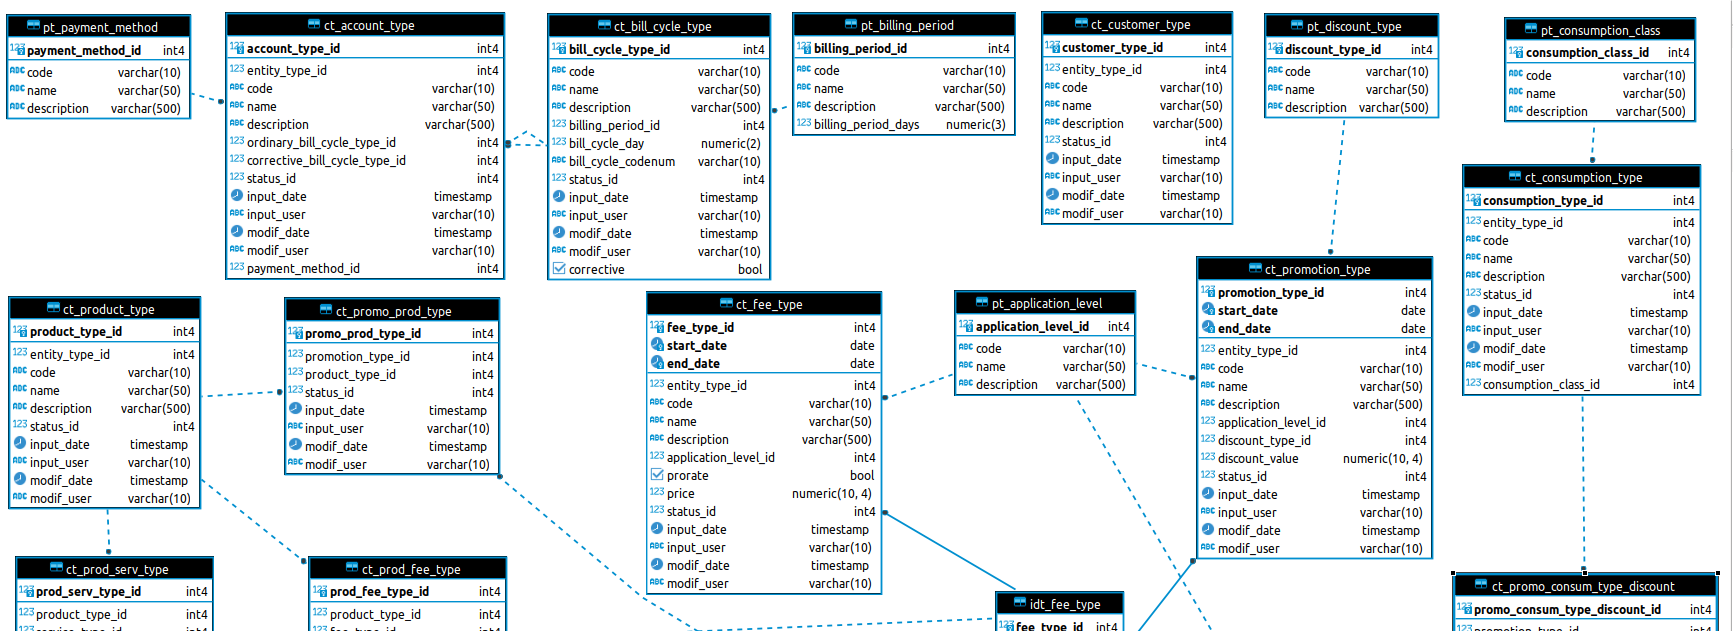
\includegraphics[width=1\textwidth]{imaxes/er-catalogo-01.png}          	  \caption{Diagrama ER del catálogo y la parametrizacion (I)}
  \label{fig:er-catalogo-01}
\end{figure}

\begin{figure}[hp!]
  \centering
  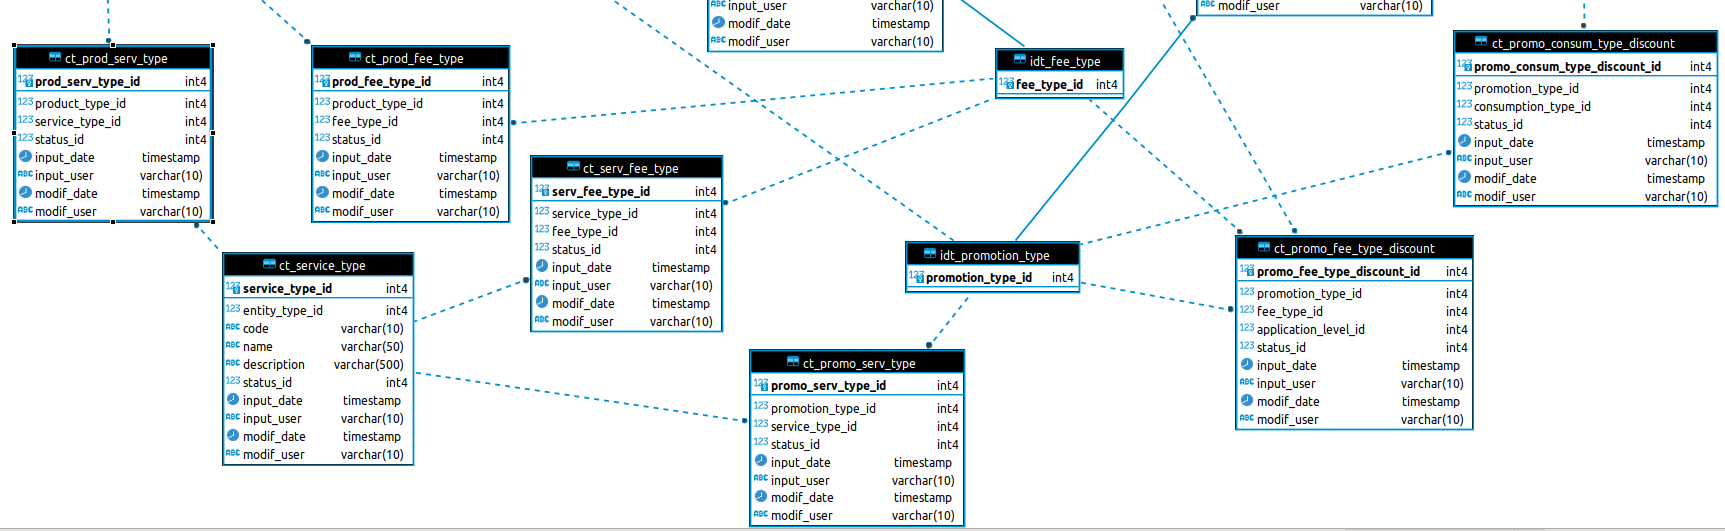
\includegraphics[width=1\textwidth]{imaxes/er-catalogo-02.png}
  \caption{Diagrama ER del catálogo y la parametrizacion (y II)}
  \label{fig:er-catalogo-02}
\end{figure}


\end{landscape}

\begin{landscape}

\begin{figure}[hp!]
  \centering
  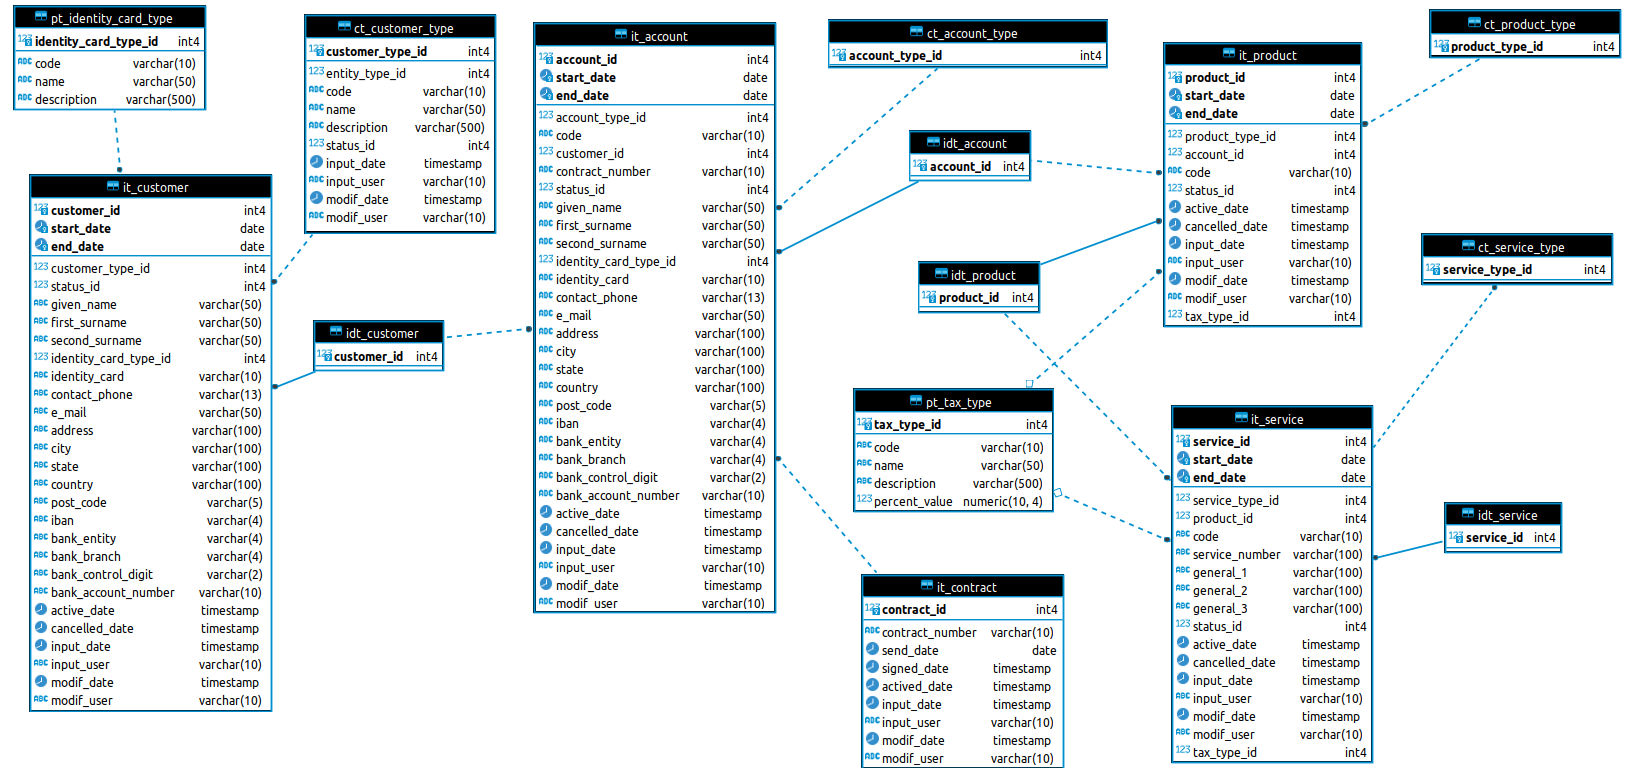
\includegraphics[width=1\textwidth]{imaxes/er-instancia-01.png}          	  \caption{Diagrama ER de la contratación, el catálogo y la parametrizacion (I)}
  \label{fig:er-instancia-01}
\end{figure}

\begin{figure}[hp!]
  \centering
  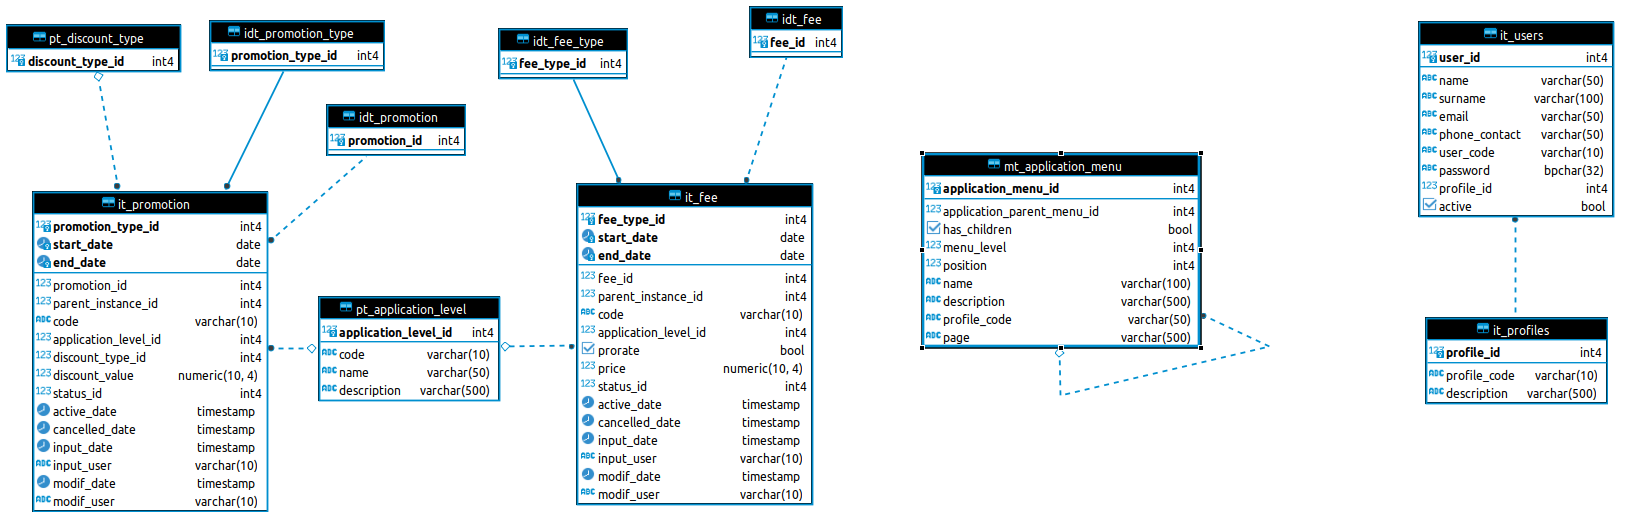
\includegraphics[width=1\textwidth]{imaxes/er-instancia-02.png}
  \caption{Diagrama ER de la contratación, el catálogo y la parametrizacion(y II)}
  \label{fig:er-instancia-02}
\end{figure}


\end{landscape}


\section{Estructura del código}
\label{chap:estructuraCodigo}

El código presentado está totalmente accesible en el siguiente repositorio de Github \url{https://github.com/cgcgit/CoMaSw.git}, bajo la carpeta CoMaSw.

El proyecto se ha desarrollado usando Maven, por lo que la estructura del mismo es la siguiente:


\begin{table} [H]
    \centering
    \rowcolors{2}{white}{white}
    \setlength{\leftmargini}{0.4cm}
	\resizebox{14cm}{!} { % evita que la tabla sobresalga de la p\'agina, ajustando tama\'no de letra y grosor de l\'ineas
    \begin{tabular}{| m{4.5cm} | m{9.5cm} |}   
    \hline
	  \textbf{Carpeta} & \textbf{Descripción} 
	  \\\hline
	  \textbf{CoMaSw} & Carpeta raíz de la aplicación. Contiene el fichero \textit{\textbf{pom.xml}}, encargado de indicar las diferentes dependencias a nivel de proyecto, posibles tareas que se pueden realizar con el proyecto (compilar, desplegar, etc), así como los módulos de los que puede constar un proyecto.
	  \\\hline
	  \textbf{CoMaSw/src/main/java} & Carpeta que almacena los distintos paquetes generados para la aplicación
	  \\\hline
	  \textbf{CoMaSw/src/main/resources} & Carpeta que almacena distintos recursos de la aplicación.
	  \\\hline
	  \textbf{CoMaSw/src/main/webapp} & Carpeta que almacena las páginas \acrshort{xhtml} y ficheros de configuración orientados a la web.
	  \\\hline
	  \textbf{CoMaSwtarget/generated-sources/jooq} & Carpeta que almacena la información relativa a las páginas web.
	  \\\hline
    \end{tabular}
    } % end /resizebox
    \caption{}
    \label{tab:estructura-codigo}
\end{table}


A continuación se detalla el contenido de las distintas carpetas.

\subsection{Directorio /src/main/java - Clases de la aplicación}
\label{sub:clases}
El directorio \textit{\textbf{/src/main/java}} contiene las clases de la aplicación agrupadas por paquetes



\begin{longtable}{m{3cm} m{12cm}}
    \caption{Paquetes con las clases de la aplicación}
    \label{tab:paquetes}\\
    \rowcolors{2}{white}{white}
    \textbf{Paquete} & \textit{\textbf{com.comasw.ejb.catalog.type}} \newline
    \acrshort{ejb} que manejan las distintas transacciones de los elementos del catálogo (obtención de datos y operaciones \acrshort{crud}).\newline
\textit{PromotionTypeEJBLocal.java},
\textit{CustomerTypeEJBLocal.java},
\textit{ProductTypeEJBLocal.java},
\textit{ConsumptionTypeEJBLocal.java},
\textit{BillCycleTypeEJBLocal.java},
\textit{ServiceTypeEJBLocal.java},
\textit{AccountTypeEJBLocal.java},
\textit{FeeTypeEJBLocal.java},
\textit{AccountTypeEJB.java},
\textit{BillCycleTypeEJB.java},
\textit{ConsumptionTypeEJB.java},
\textit{CustomerTypeEJB.java},
\textit{FeeTypeEJB.java},
\textit{ProductTypeEJB.java},
\textit{PromotionTypeEJB.java},
\textit{ServiceTypeEJB.java}.
    \\\hline
    \textbf{Paquete} & \textit{\textbf{com.comasw.ejb.catalog.relationType}} \newline
     \acrshort{ejb} que manejan las distintas transacciones de las relaciones entre los distintos elementos del catálogo (obtención de datos y operaciones \acrshort{crud}).\newline
\textit{ProductFeeTypeEJBLocal.java},
\textit{ProductPromotionTypeEJBLocal.java},
\textit{ProductFeeTypeEJB.java},
\textit{ProductServiceTypeEJBLocal.java},
\textit{PromotionConsumptionTypeDiscountEJBLocal.java},
\textit{PromotionFeeTypeDiscountEJBLocal.java},
\textit{ServiceFeeTypeEJBLocal.java},
\textit{ServicePromotionTypeEJBLocal.java},
\textit{ProductPromotionTypeEJB.java},
\textit{ProductServiceTypeEJB.java},
\textit{PromotionConsumptionTypeDiscountEJB.java},
\textit{PromotionFeeTypeDiscountEJB.java},
\textit{ServiceFeeTypeEJB.java},
\textit{ServicePromotionTypeEJB.java}.
	\\\hline
	\textbf{Paquete} & \textit{\textbf{com.comasw.ejb.user}} \newline
     \acrshort{ejb} que manejan las distintas transacciones de usuarios y perfiles (obtención de datos y operaciones \acrshort{crud}).\newline
\textit{ProfileEJBLocal.java},
\textit{ApplicationUserEJBLocal.java},
\textit{ProfileEJB.java},
\textit{ApplicationUserEJB.java}.
	\\\hline
	\textbf{Paquete} & \textit{\textbf{com.comasw.ejb.parameterization}} \newline
     \acrshort{ejb} que manejan las distintas transacciones de los elementos de la parametrización (obtención de datos y operaciones \acrshort{crud}).\newline
\textit{EntityTypeEJBLocal.java},
\textit{BillingPeriodEJBLocal.java},
\textit{PaymentMethodEJBLocal.java},
\textit{TaxTypeEJBLocal.java},
\textit{DiscountTypeEJBLocal.java},
\textit{ConsumptionClassEJBLocal.java},
\textit{ApplicationLevelEJBLocal.java},
\textit{IdentityCardTypeEJBLocal.java},
\textit{StatusEJBLocal.java},
\textit{ApplicationLevelEJB.java},
\textit{BillingPeriodEJB.java},
\textit{ConsumptionClassEJB.java},
\textit{DiscountTypeEJB.java},
\textit{IdentityCardTypeEJB.java},
\textit{PaymentMethodEJB.java},
\textit{StatusEJB.java},
\textit{TaxTypeEJB.java},
\textit{EntityTypeEJB.java}.
	\\\hline

	\textbf{Paquete} & \textit{\textbf{com.comasw.ejb.instance}} \newline
    Los EJB que manejan las distintas transacciones de los elementos de las instancias/contrataciones (obtención de datos y operaciones \acrshort{crud}). \newline
\textit{ContractEJBLocal.java},
\textit{ContractEJB.java},
\textit{AccountEJBLocal.java},
\textit{ProductEJBLocal.java},
\textit{ServiceEJBLocal.java},
\textit{PromotionEJBLocal.java},
\textit{FeeEJBLocal.java},
\textit{CustomerEJBLocal.java},
\textit{AccountEJB.java},
\textit{FeeEJB.java},
\textit{ProductEJB.java},
\textit{PromotionEJB.java},
\textit{ServiceEJB.java},
\textit{CustomerEJB.java}.
	\\\hline

	\textbf{Paquete} & \textit{\textbf{com.comasw.ejb.miscelaneous}} \newline
     \acrshort{ejb} que manejan las distintas transacciones de para otros elementos (obtención de datos y operaciones \acrshort{crud}).\newline
\textit{ApplicationMenuEJBLocal.java},
\textit{ApplicationMenuEJB.java}.
	\\\hline

\textbf{Paquete} & \textit{\textbf{com.comasw.viewController.parameterization}} \newline
     Controlador para la vistas relativas a los elementos de parametrización.\newline
\textit{ApplicationLevelController.java},
\textit{BillingPeriodController.java},
\textit{ConsumptionClassController.java},
\textit{DiscountTypeController.java},
\textit{EntityTypeController.java},
\textit{IdentityCardTypeController.java},
\textit{PaymentMethodController.java},
\textit{StatusController.java},
\textit{TaxTypeController.java}.

	\\\hline
\textbf{Paquete} & \textit{\textbf{com.comasw.viewController.catalog.type}} \newline
     Controlador para las vistas relativas al catálogo.\newline
\textit{AccountTypeController.java},
\textit{BillCycleTypeController.java},
\textit{ConsumptionTypeController.java},
\textit{CustomerTypeController.java},
\textit{ProductTypeController.java},
\textit{ServiceTypeController.java},
\textit{PromotionTypeController.java},
\textit{FeeTypeController.java}.
	\\\hline

	\textbf{Paquete} & \textit{\textbf{com.comasw.viewController.catalog.relationType}} \newline
     Controlador para las vistas relativas a las relaciones del catálogo.\newline
\textit{ProductServiceTypeController.java},
\textit{ProductFeeTypeController.java},
\textit{PromotionConsumptionTypeDiscController.java},
\textit{ProductPromotionTypeController.java},
\textit{ServicePromotionTypeController.java},
\textit{ServiceFeeTypeController.java},
\textit{PromotionFeeTypeDiscountController.java}.
	\\\hline


\textbf{Paquete} & \textit{\textbf{com.comasw.viewController.instance}} \newline
     Controlador para la vistas relativas a los elementos de las contrataciones (instancias).\newline
\textit{AccountController.java},
\textit{ContractController.java},
\textit{CustomerController.java},
\textit{FeeController.java},
\textit{HierarchyController.java},
\textit{ProductController.java},
\textit{PromotionController.java},
\textit{ServiceController.java}.
	\\\hline


	\textbf{Paquete} & \textit{\textbf{com.comasw.viewController.templateController}} \newline
     Controlador para la plantilla de las vistas.\newline
\textit{MainTemplateController.java}.
	\\\hline


\textbf{Paquete} & \textit{\textbf{com.comasw.viewController.appAccessController}} \newline
     Controlador para el inicio y fin de sesión y la definición del menu en función de los permisos del usuario que ha accedido a la aplicación.\newline
\textit{LogoutController.java},
\textit{LoginController.java},
\textit{ApplicationMenuController.java}.
	\\\hline


	\textbf{Paquete} & \textit{\textbf{com.comasw.viewController.user}} \newline
     Controladores para la gestión de usuarios.\newline
\textit{UserProfileController.java},
\textit{ManageUserController.java}.
	\\\hline

	\textbf{Paquete} & \textit{\textbf{com.comasw.auth}} \newline
     Clases que gestionan el acceso y la autenticación de usuarios.\newline
\textit{ApplicationConfig.java},
\textit{UserServiceIdentityStore.java}.
	\\\hline

	\textbf{Paquete} & \textit{\textbf{com.comasw.converter}} \newline
     Clases para la conversión de datos en \acrshort{jsf}.\newline
\textit{LocalDateTimeConverter.java}.
	\\\hline

	\textbf{Paquete} & \textit{\textbf{com.comasw.exception}} \newline
     Clases para el manejo de excepciones de la aplicación.\newline
\textit{CoMaSwDataAccessException.java},
\textit{CoMaSwGeneralException.java},
\textit{CoMaSwParseException.java}.
	\\\hline

	\textbf{Paquete} & \textit{\textbf{com.comasw.generalClass}} \newline
     Clases extienden a las clases controladoras.\newline
\textit{BasicClass.java},
\textit{BasicHistoricType.java},
\textit{BasicInstance.java},
\textit{BasicInstanceWithViews.java},
\textit{BasicListsForInstance.java},
\textit{BasicRelationType.java},
\textit{BasicType.java},
\textit{BasicTypeWithLists.java},
\textit{ClassWithLists.java},
\textit{DoubleHistoricRelation.java},
\textit{RelatedInstance.java},
\textit{SimpleHistoricRelation.java}.
	\\\hline

	\textbf{Paquete} & \textit{\textbf{com.comasw.interfaces}} \newline
     Interfaces a implementar por las clases controladoras.\newline
\textit{IDoubleHistoricRelationsTable.java},
\textit{IEditableHistoricTable.java},
\textit{IEditableTable.java},
\textit{IHistoricTable.java},
\textit{IInstanceTable.java},
\textit{IRelationsTable.java},
\textit{ISimpleHistoricRelationsTable.java},
\textit{ITableAdd.java},
\textit{ITable.java}.
	\\\hline

	\textbf{Paquete} & \textit{\textbf{com.comasw.utilities}} \newline
     Clases que contienen distintas utilidades usadas por los controladores.\newline
\textit{Formatter.java},
\textit{Messages.java},
\textit{Utilities.java}.
	\\\hline


	\textbf{Paquete} & \textit{\textbf{com.comasw.utilities}} \newline
     Clases validadoras usadas por las vistas \acrshort{jsf}.\newline
\textit{EndDateValidator.java},
\textit{StartDateValidator.java}.
	\\\hline


\end{longtable}

 


\subsection{Directorio /src/main/webapp}
\label{sub:web}
Además de contener las páginas \acrshort{xhtml} de login y error, contiene la siguiente información:


\begin{longtable}{m{3cm} m{12cm}}
    \caption{Directorio webapp}
    \label{tab:web}\\  	
    \rowcolors{2}{white}{white}
    \textbf{carpeta} & \textit{\textbf{app}} \newline
    Contiene las distintas páginas \acrshort{xhtml} que definen las vistas de la aplicación.
    \\\hline
    \textbf{carpeta} & \textit{\textbf{WEB-INF}} \newline
    Archivos de configuración y plantilla usada en las vistas de la aplicación.
	\\\hline
\\\hline

\end{longtable}    
 


\subsection{Directorio /src/main/resources - Recursos de la aplicacion}
\label{sub:recursos-aplicacion}
El directorio \textit{\textbf{/src/main/resources}} contiene los distintos recursos usados por la aplicación. A continuación se ofrece un listado del contenido del mismo.


\begin{longtable}{m{3cm} m{12cm}}
    \caption{Recursos}
    \label{tab:recursos}\\  	
    \rowcolors{2}{white}{white}
    \textbf{Paquete} & \textit{\textbf{com.comasw.properties}} \newline
    Ficheros que contienen las distintas propiedades utilizadas en la aplicación.\newline
    \textit{dataBaseDefinitions.properties} que contiene información relevante para la identificación de ciertos elementos en la base de datos,
\textit{modifyingProfile.properties} que indica si un perfil tiene o no asociada la funcionalidad de creación y edición de información.
\textit{pageTitle.properties} que contiene el nombre de las distintas páginas \acrshort{xhtml} creadas.
\textit{uiValues.properties} que contiene valores genéricos de componentes usados en las páginas \acrshort{xhtml}.
\textit{urlPage.properties} que contiene informaciones relativas a distintas urls.
\\\hline
	\textbf{Carpeta} & \textit{\textbf{Documentation}} \newline
    Contiene lo siguiente:
    \begin{itemize}
    \item Carpeta instalationFiles, que contiene el fichero \emph{comasw\_files.zip} con todos los ficheros necesarios para instalar la aplicaicón y el fichero readme.txt con los pasos a seguir.
    \item Fichero \emph{manual\_usuario.pdf} con el manual de usuario de la aplicación.
    \item Fichero \emph{db\_comasw\_html.zip} con la documentación de la base de datos comasw en formato html.
    \end{itemize}    
    \\\hline
	\textbf{Carpeta} & \textit{\textbf{License}} \newline
	Contiene el fichero \emph{\textbf{gpl-3.0.txt}} que conitene la licencia bajo el que se ha desarrollado la aplicación (\acrshort{licencia}).
    \\\hline
	\textbf{Fichero} & \textit{\textbf{log4j2.xml}} \newline
    Fichero de configuración de Log4j.
	\\\hline
	\textbf{Carpeta} & \textit{\textbf{META-INF}} \newline
    Contiene el fichero persistence.xml.
	\\\hline
\\\hline

\end{longtable}    



\subsection{Directorio /target/generated-sources/jooq - Clases generadas}
\label{sub:clases-generadas}
El directorio \textit{\textbf{/target/generated-sources/jooq}} contiene las distintas clases generadas por el generador de clases de \acrshort{jooq}. A continuación se presenta el listado con el contenido del mismo



\begin{longtable}{m{3cm} m{12cm}}
    \caption{Clases generadas}
    \label{tab:generados}\\  	
    \rowcolors{2}{white}{white}
\textbf{Paquete} & \textit{\textbf{com/comasw/model}} \newline
	Contiene las distintas clases que definen la base de datos.\newline    
\textit{DefaultCatalog.java}, 
\textit{Keys.java}, 
\textit{Public.java}, 
\textit{Routines.java}, 
\textit{Sequences.java}, 
\textit{Tables.java},
\\\hline

	\textbf{Paquete} & \textit{\textbf{com.comasw.model.tables}} \newline
	Contiene las distintas clases que definen las distintas tablas y vistas de la base de datos.\newline
\textit{CtAccountType.java}, 
\textit{CtBillCycleType.java}, 
\textit{CtConsumptionType.java}, 
\textit{CtCustomerType.java}, 
\textit{CtFeeType.java}, 
\textit{CtProdFeeType.java}, 
\textit{CtProdServType.java}, 
\textit{CtProductType.java}, 
\textit{CtPromoConsumTypeDiscount.java}, 
\textit{CtPromoFeeTypeDiscount.java}, 
\textit{CtPromoProdType.java}, 
\textit{CtPromoServType.java}, 
\textit{CtPromotionType.java}, 
\textit{CtServFeeType.java}, 
\textit{CtServiceType.java}, 
\textit{IdtAccount.java}, 
\textit{IdtCustomer.java}, 
\textit{IdtFee.java}, 
\textit{IdtFeeType.java}, 
\textit{IdtProductFee.java}, 
\textit{IdtProduct.java}, 
\textit{IdtProductPromotion.java}, 
\textit{IdtProductService.java}, 
\textit{IdtPromotion.java}, 
\textit{IdtPromotionType.java}, 
\textit{IdtServiceFee.java}, 
\textit{IdtService.java}, 
\textit{IdtServicePromotion.java}, 
\textit{ItAccount.java}, 
\textit{ItContract.java}, 
\textit{ItCustomer.java}, 
\textit{ItFee.java}, 
\textit{ItProduct.java}, 
\textit{ItProfiles.java}, 
\textit{ItPromotion.java}, 
\textit{ItService.java}, 
\textit{ItUsers.java}, 
\textit{MtApplicationMenu.java}, 
\textit{PtApplicationLevel.java}, 
\textit{PtBillingPeriod.java}, 
\textit{PtConsumptionClass.java}, 
\textit{PtDiscountType.java}, 
\textit{PtEntityType.java}, 
\textit{PtIdentityCardType.java}, 
\textit{PtPaymentMethod.java}, 
\textit{PtStatus.java}, 
\textit{PtTaxType.java}, 
\textit{VwAccountInstance.java}, 
\textit{VwCustomerInstance.java}, 
\textit{VwFeeInstance.java}, 
\textit{VwProductFeeType.java} ,
\textit{VwProductInstance.java}, 
\textit{VwProductServiceType.java}, 
\textit{VwPromoConsumTypeDiscount.java}, 
\textit{VwPromotionFeeTypeDiscount.java}, 
\textit{VwPromotionInstance.java}, 
\textit{VwPromotionProductType.java}, 
\textit{VwPromotionServiceType.java}, 
\textit{VwServiceFeeType.java}, 
\textit{VwServiceInstance.java}, 
\textit{VwUsers.java}.
 \\\hline
	\textbf{Paquete} & \textit{\textbf{com.comasw.model.tables.pojos}}\newline
	Clases POJO de las distintas tablas de la aplicación.
\\\hline
	\textbf{Paquete} & \textit{\textbf{com.comasw.model.tables.daos}}\newline
	Clases DAO de las distintas tablas de la aplicación.
\\\hline
	\textbf{Paquete} & \textit{\textbf{com.comasw.model.tables.record}}\newline
	Clases RECORD de las distintas tablas de la aplicación.
\\\hline
	\textbf{Paquete} & \textit{\textbf{com.comasw.model.tables.interfaces}}\newline
	Interfaces para distintas tablas de la aplicación.
\\\hline

\end{longtable}    